%%!TEX root = ./marylie.tex
%%--.----1----.----2----.----3----.----4----.----5----.----6----.----7----.-!

\chapter{Catalog of Beam-Line Elements}
     The beam-line elements and their type code mnemonics, as currently
available in \Mary 3.0, are listed below.\index{beam-line elements} \index{element library} \index{catalog}  Also listed are the
subsections that describe them in detail.

\begin{center}
\begin{tabular}{lll}
\multicolumn{1}{c}{\underline{Type Code}} &
\multicolumn{1}{c}{\underline{Element}}   &
\multicolumn{1}{c}{\underline{Subsection}} \\
\hspace{1.5em}drft    &         Drift Space                         &  \hspace{2em}6.1 \\
\vspace{-3mm}& &\\
               &         \underline{Dipole Bend Magnets}    &      \\
\vspace{-3mm}& &\\
\hspace{1.5em}nbnd   &   \makebox[1em][l]{a)} Normal Entry Bending Magnet,    &  \hspace{2em}6.2 \\
               &   \hspace*{1em} with or without Fringe Fields.  &      \\
\vspace{-3mm}& &\\
\hspace{1.5em}pbnd    &  \makebox[1em][l]{b)} Parallel Faced Bending Magnet,  &  \hspace{2em}6.3 \\
               &   \hspace*{1em}   with Fringe Fields and equal    &      \\
               &   \hspace*{1em}  entry and exit angles.          &      \\
\vspace{-3mm}& &\\
\hspace{1.5em}gbnd    &         c)  General Bending Magnet.         &  \hspace{2em}6.4 \\
\vspace{-3mm}& &\\
\hspace{1.5em}prot    &   \makebox[1em][l]{d)} Used for Leading and Trailing   &  \hspace{2em}6.5 \\
               &  \hspace*{1em}           Pole Face Rotations.            &      \\
\vspace{-3mm}& &\\
\hspace{1.5em}gbdy    &   \makebox[1em][l]{e)} Used for the Body of a General  &  \hspace{2em}6.6 \\
               &  \hspace*{1em} Bending Magnet.                 &      \\
\vspace{-3mm}& &\\
\hspace{1.5em}frng    & f)  Used for Hard-Edge Dipole Fringe Fields. &  \hspace{2em}6.7 \\
\vspace{-3mm}& &\\
\hspace{1.5em}cfbd    &         g)  Combined Function Bend.         &  \hspace{2em}6.8 \\
\vspace{-3mm}& &\\
\hspace{1.5em}quad    &         Magnetic Quadrupole.                 &  \hspace{2em}6.9 \\
\vspace{-3mm}& &\\
\hspace{1.5em}sext    &         Magnetic Sextupole.         &  \hspace{2em}6.10\\
\vspace{-3mm}& &\\
\hspace{1.5em}octm    &         Magnetic Octupole.                   &  \hspace{2em}6.11\\
\vspace{-3mm}& &\\
\hspace{1.5em}octe    &         Electric Octupole.                   &  \hspace{2em}6.12
\end{tabular}

\begin{tabular}{lll}
\multicolumn{1}{c}{\underline{Type Code}} &
\multicolumn{1}{c}{\underline{Element}}   &
\multicolumn{1}{c}{\underline{Subsection}} \\
\hspace{1.5em}srfc    &         Short RF Cavity.                    &  \hspace{2em}6.13\\
\vspace{-3mm}& &\\
\hspace{1.5em}arot    &         Axial Rotation.                      &  \hspace{2em}6.14\\
\vspace{-3mm}& &\\
\hspace{1.5em}twsm    &      Linear matrix transformation specified &  \hspace{2em}6.15\\
               &         in terms of twiss parameters.        &      \\
\vspace{-3mm}& &\\
\hspace{1.5em}thlm    &         ``Thin lens'' approximation to low    &\hspace{2em}6.16\\
               &         order multipoles.                    &      \\
\vspace{-3mm}& &\\
\hspace{1.5em}cplm    &         ``Compressed'' approximation to low   &\hspace{2em}6.17\\
               &         order multipoles.                    &      \\
\vspace{-3mm}& &\\
\hspace{1.5em}jmap    &         Map with matrix part J.              &  \hspace{2em}6.18\\
\vspace{-3mm}& &\\
\hspace{1.5em}r****   &         Random counterpart of the element   &  \hspace{2em}6.19\\
               &         with type-code mnemonic ****.        &      \\
\vspace{-3mm}& &\\
\hspace{1.5em}usr1    &         User Specified Subroutines that     &  \hspace{2em}6.20\\
\vspace{-7mm}& &\\
\hspace{1.5em}\ \ \,$\vdots$ &         act on phase space data.             &      \\
\vspace{-7mm}& &\\
\hspace{1.5em}usr10    &                                             &      \\
\vspace{-3mm}& &\\
\hspace{1.5em}usr11    &         User Specified Subroutines that     &  \hspace{2em}6.21\\
\vspace{-7mm}& &\\
\hspace{1.5em}\ \ \,$\vdots$ &         produce or act on maps.              &      \\
\vspace{-7mm}& &\\
\hspace{1.5em}usr20    &                                             &      \\
\vspace{-3mm}& &\\
\hspace{1.5em}dism    &         Dispersion matrix.                   &  \hspace{2em}6.22\\
\vspace{-3mm}& &\\
\hspace{1.5em}sol    &         Solenoid.                            &  \hspace{2em}6.23\\
\vspace{-3mm}& &\\
\hspace{1.5em}cfqd    &       Combined Function Magnetic Quadrupole. &  \hspace{2em}6.24\\
\vspace{-3mm}& &\\
\hspace{1.5em}mark    &         Marker.                              &  \hspace{2em}6.25\\
\vspace{-3mm}& &\\
\hspace{1.5em}dp      &         Data Point.                          &  \hspace{2em}6.26\\
\vspace{-3mm}& &\\
\hspace{1.5em}recm    &         REC Quadrupole Multiplet.              & \hspace{2em}6.27\\
\vspace{-3mm}& &\\
\hspace{1.5em}spce    &         Space for accounting purposes.       & \hspace{2em}6.28\\
\vspace{-3mm}& &\\
\hspace{1.5em}cfrn    & Change or write out values of fringe field parameters& \hspace{2em}6.29\\
                      & for combined function dipole.                    &      \\
\vspace{-3mm}& &\\
\hspace{1.5em}rmap    &         Random map.       & \hspace{2em}6.30\\
\hspace{1.5em}arc    &  Angular space for accounting purposes.   & \hspace{2em}6.31
\end{tabular}
\end{center}
Note that the type codes are given in lower case.  If entries are made in
upper case, they are automatically converted to lower case by PREP and
\Maryend.

     The purpose of this section is to outline the use of these elements by
\Maryend, and to describe the parameters required to specify these elements
in the \#menu component of the Master Input File.

     Calculations of $f_2$  (or equivalently the matrix $R$), $f_3$ , and $f_4$  for the
beam-line elements listed in this section have been carried out by Diamond, Douglas,
Dragt, Forest, Healy, Neri, Ryne, and van Zeijts.  Expressions for the coefficients
of the various polynomials may be found in the papers listed in Chapter 11.  It is expected that other elements, some of which may
be described through $4^{\mbox{\scriptsize th}}$ and $5^{\mbox{\scriptsize th}}$ order in terms of polynomials $f_5$  and $f_6$,
will be added to \Maryend 's library in the future.

\newpage
\section{Drift}
\begin{quotation}
\noindent Type Code:  drft
\vspace{5mm}

\noindent Required Parameters:
\begin{enumerate}
     \item  Length of drift (m).
\end{enumerate}

\vspace{5mm}
\noindent    Example:
\begin{verbatim}
         dr5   drft
         0.3D+01
\end{verbatim}
\end{quotation}
The above specifies a drift space with user given name {\em dr5}, and length
3 meters.\index{drift}  For an example of a \Mary run that computes and displays the
transfer map for a drift, see section 3.11.1.

\newpage
\section{Normal Entry and Exit (Sector) Bending Magnet}
\begin{quotation}
\noindent Type Code:  nbnd or sbnd
\vspace{5mm}

\noindent Required Parameters:
\begin{enumerate}
      \item  Bend angle in degrees.
      \item  Gap size (pole to pole distance) in meters.
      \item  Normalized field integral (dimensionless).
      \item  Magnetic field, B (Tesla).
      \item  LFRN

             \ = 0 for no fringe field on leading edge (entry) of dipole.

             \ = 1 for hard-edge fringe field on leading edge of dipole.
      \item  TFRN

             \ = 0 for no fringe field on trailing edge (exit) of dipole.

             \ = 1 for hard-edge fringe field on trailing edge of dipole.
\end{enumerate}

\vspace{5mm}
\noindent     Example:
\begin{verbatim}
         bend   nbnd
         36., .03, .5, l.2, 1, 1
\end{verbatim}
\end{quotation}
This specifies a normal entry bend with user given name {\em bend }.\index{bending magnet} \index{dipole}  It subtends
an angle of $36^{\circ}$, has a field of 1.2 Tesla, and has leading and trailing
hard-edge fringe fields.  The full gap size (pole to pole distance) is .03 meters,
and the normalized field integral is .5.

\vspace{5mm}
     Vector potential:  ${\displaystyle A_{\phi}  = -\frac{\rho B}{2}}$.

\vspace{5mm}
     Description:
\vspace{2mm}

     The type code {\em nbnd } produces a normal entry (sector) dipole that bends to the right.
See figures 6.2.1 through 6.2.3 and Exhibit 6.2.1.  Normal entry dipoles that bend
in other directions may be obtained by using {\em nbnd} in conjunction with
{\em arot}.  See figures 6.2.4 through 6.2.7 and Exhibits 6.2.2 through 6.2.6
for various kinds of normal entry bends and their associated coordinate
systems.  For the benefit of those accustomed to referring to such
magnets as {\em sector bends}, \Mary also recognizes the equivalent type code
mnemonic {\em sbnd}.

        For analytic calculations, trajectories in figure 6.2.1 can be conveniently
computed using the right handed cylindrical triad ${\bf e}_{\rho}, {\bf e}_y,
{\bf e}_{\phi}$.  Note that this choice differs from the more familiar
right-handed triad ${\bf e}_{\rho}, {\bf e}_{\phi}, {\bf e}_z$.  For example,
one finds the results

\pagebreak

\begin{eqnarray*}
  B_{\rho} & = (\nabla \times {\bf A})_{\rho} & = \frac{\partial A_{\phi}}{\partial y\ \ }
  - \frac{1}{\rho} \frac{\partial A_y}{\partial \phi\ \ }=0, \\
  B_y  & = (\nabla \times {\bf A})_y  & = \frac{1}{\rho}\frac{\partial A_{\rho}}{\partial\phi\ \ }-\frac{1}{\rho}\frac{\partial\ }{\partial \rho}
(\rho A_{\phi})\\
       &{\displaystyle = \frac{1}{\rho} \frac{\partial\ }{\partial \rho} (\frac{\rho ^2
B}{2}) }& = B, \\
  B_{\phi} & = (\nabla \times {\bf A})_{\phi} & = \frac{\partial A_y}{\partial \rho\ \ } -
  \frac{\partial A_{\rho}}{\partial y\ \ } = 0.
\end{eqnarray*}


     Leading and trailing fringe fields, when employed, are treated in the
finite gap approximation.  In the absence of better information, the normalized field integral parameter should be set equal to .5.  For a further discussion of the finite gap approximation, see section 6.7.

\begin{figure}[hp]
  \centering
  \includegraphics[scale=0.453]{EntryBendTop}
  \caption{Geometry of a Normal Entry Bend, top view.
A positive particle is bent to the right (the $-x$ direction).  The bend
angle is $\theta$.  The bending radius $\rho$, path length $s$, and cord length $d$ are
given by the relations}
\[  \rho = \frac{B\rho}{B},\ s = \rho\theta,\ d=2\rho\sin(\frac{\theta}{2}). \nonumber \]
\end{figure}

\begin{figure}[hp]
  \centering
  \includegraphics[scale=0.453]{EntryBendEnd}
  \caption{Geometry of a Normal Entry Bend, end view.
The magnetic field $B$ is along the $+y$ direction, and the magnetic force $F$ on
a positive particle is in the $-x$ direction.  If the magnetic field is
viewed as being produced by poles, then the south pole is above and the
north pole is below as shown.  (Recall that magnetic field lines come out of north poles and go into south poles.)}
\end{figure}

\begin{figure}[hp]
  \centering
  \includegraphics[scale=0.453]{EntryBendOrbits}
  \caption{Illustrative off energy orbits (for a positive particle) in a
Normal Entry Bend (top view).  A normal entry particle exits with $x > 0$ if
the energy exceeds the design energy ($P_{\tau}< 0$), and exits with $x < 0$ if the
energy is below the design energy ($P_{\tau}> 0$).  See Exhibit 6.2.1.}
\end{figure}

\begin{figure}[hp]
  \centering
  \includegraphics[scale=0.453]{EntryBendLeft}
  \caption{Geometry of a Normal Entry Bend that bends a positive
particle to the left (top view).  It is obtained by using the type code
{\em nbnd } preceded and followed by axial rotations of $+180^\circ$ and $-180^\circ$,
respectively.  See Exhibit 6.2.2.  Alternatively, the same effect can be
achieved by using {\em nbnd } alone with $\theta < 0$ and $B < 0$.  See Exhibit 6.2.3.}
\end{figure}


\begin{figure}[hp]
  \centering
  \includegraphics[scale=0.453]{EntryBendUp}
  \caption{Geometry of a vertical Normal Entry Bend (side view) that
bends a positive particle up.  It is obtained by using the type code {\em nbnd }
preceded and followed by axial rotations of $+90^\circ$ and $-90^\circ$,
respectively.  See Exhibit 6.2.4.}
\end{figure}

\begin{figure}[hp]
  \centering
  \includegraphics[scale=0.453]{EntryBendDown}
  \caption{Geometry of a vertical Normal Entry Bend (side view) that
bends a positive particle down.  It is obtained by using the type code {\em nbnd }
preceded and followed by axial rotations of $-90^\circ$ and $+90^\circ$,
respectively.  See Exhibit 6.2.5.}
\end{figure}


\begin{figure}[hp]
  \centering
  \includegraphics[scale=0.453]{UpwardStep}
  \caption{Geometry (side view) of a vertical upward ``step'' (for
positive particles) employing two Normal Entry Bends separated by a Drift.
See Exhibit 6.2.6.}
\end{figure}


\clearpage
\begin{footnotesize}
\begin{verbatim}
#comment
 Exhibit 6.2.1.
 This is a MARYLIE run illustrating the sign conventions for a
 Normal Entry Bend rbend that bends to the right.
 The beam parameters are those for 800 MeV protons.
#beam
  4.881030646470486
 0.8526309382400936
  1.000000000000000
  1.000000000000000
#menu
 fileout  pmif
   1.00000000000000       12.0000000000000       3.00000000000000
 matout   ptm
   3.00000000000000      0.000000000000000E+00  0.000000000000000E+00
  0.000000000000000E+00   1.00000000000000
 raysin   rt
   13.0000000000000       14.0000000000000      -1.00000000000000
  0.000000000000000E+00  0.000000000000000E+00  0.000000000000000E+00
 trace    rt
  0.000000000000000E+00   14.0000000000000       4.00000000000000
  0.000000000000000E+00   1.00000000000000      0.000000000000000E+00
 rbend    nbnd
   36.0000000000000      0.000000000000000E+00  0.500000000000000
   1.20000000000000       1.00000000000000       1.00000000000000
 end      end
#labor
    1*fileout
    1*rbend
    1*matout
    1*raysin
    1*trace
    1*end

matrix for map is :

 8.09017E-01  2.39083E+00  0.00000E+00  0.00000E+00  0.00000E+00 -9.22806E-01
-1.44507E-01  8.09017E-01  0.00000E+00  0.00000E+00  0.00000E+00 -6.98239E-01
 0.00000E+00  0.00000E+00  1.00000E+00  2.55570E+00  0.00000E+00  0.00000E+00
 0.00000E+00  0.00000E+00  0.00000E+00  1.00000E+00  0.00000E+00  0.00000E+00
 6.98239E-01  9.22806E-01  0.00000E+00  0.00000E+00  1.00000E+00  8.18104E-01
 0.00000E+00  0.00000E+00  0.00000E+00  0.00000E+00  0.00000E+00  1.00000E+00
\end{verbatim}
\end{footnotesize}
Initial conditions for ray trace (contents of file 13):
\begin{footnotesize}
\begin{verbatim}
 0 0 0 0 0 -.01
 0 0 0 0 0 +.01
\end{verbatim}
\end{footnotesize}
Final conditions for ray trace (contents of file 14):
\begin{footnotesize}
\begin{verbatim}
 9.11465E-03  6.97045E-03  0.00000E+00  0.00000E+00 -8.00914E-03 -1.00000E-02
-9.34490E-03 -6.99462E-03  0.00000E+00  0.00000E+00  8.35945E-03  1.00000E-02
\end{verbatim}
\end{footnotesize}

\newpage
\begin{footnotesize}
\begin{verbatim}
#comment
 Exhibit 6.2.2.
 This is a MARYLIE run illustrating the sign conventions for a
 Normal Entry Bend lbnd that bends to the left.
 The element lbnd is achieved using nbnd with preceding and
 following rotations of +180 and -180 degrees, respectively.
 The beam parameters are those for 800 MeV protons.
#beam
  4.881030646470486
 0.8526309382400936
  1.000000000000000
  1.000000000000000
#menu
 fileout  pmif
   1.00000000000000       12.0000000000000       3.00000000000000
 matout   ptm
   3.00000000000000      0.000000000000000E+00  0.000000000000000E+00
  0.000000000000000E+00   1.00000000000000
 raysin   rt
   13.0000000000000       14.0000000000000      -1.00000000000000
  0.000000000000000E+00  0.000000000000000E+00  0.000000000000000E+00
 trace    rt
  0.000000000000000E+00   14.0000000000000       4.00000000000000
  0.000000000000000E+00   1.00000000000000      0.000000000000000E+00
 rbend    nbnd
   36.0000000000000      0.000000000000000E+00  0.500000000000000
   1.20000000000000       1.00000000000000       1.00000000000000
 rot+180  arot
   180.000000000000
 rot-180  arot
  -180.000000000000
 end      end
#lines
 lbend
     1*rot+180     1*rbend       1*rot-180
#lumps
#loops
#labor
    1*fileout
    1*lbend
    1*matout
    1*raysin
    1*trace
    1*end

matrix for map is :

 8.09017E-01  2.39083E+00  8.41639E-18  7.26563E-18  0.00000E+00  9.22806E-01
-1.44507E-01  8.09017E-01  6.36824E-18  8.41639E-18  0.00000E+00  6.98239E-01
 8.41639E-18  7.26563E-18  1.00000E+00  2.55570E+00  0.00000E+00 -4.06669E-17
 6.36824E-18  8.41639E-18 -2.80640E-34  1.00000E+00  0.00000E+00 -3.07705E-17
-6.98239E-01 -9.22806E-01  3.07705E-17  4.06669E-17  1.00000E+00  8.18104E-01
 0.00000E+00  0.00000E+00  0.00000E+00  0.00000E+00  0.00000E+00  1.00000E+00
\end{verbatim}
\end{footnotesize}
Initial conditions for ray trace (contents of file 13):
\begin{footnotesize}
\begin{verbatim}
 0 0 0 0 0 -.01
 0 0 0 0 0 +.01
\end{verbatim}
\end{footnotesize}
Final conditions for ray trace (contents of file 14):
\begin{footnotesize}
\begin{verbatim}
-9.11465E-03 -6.97045E-03  4.01671E-19  3.07179E-19 -8.00914E-03 -1.00000E-02
 9.34490E-03  6.99462E-03 -4.11818E-19 -3.08244E-19  8.35945E-03  1.00000E-02
\end{verbatim}
\end{footnotesize}

\newpage
\begin{footnotesize}
\begin{verbatim}
#comment
Exhibit 6.2.3.
This is a MARYLIE run illustrating that a Normal Entry Bend (lbnd or
negbend) that bends to the left can be achieved in two ways: lbnd uses
nbnd with preceding and following rotations of +180 and -180 degrees,
respectively; negbend uses nbnd with a negative bend angle and a negative
field strength.  The map (lbnd inverse)*negbend is computed, and shown to
be (to machine precision) the identity map.
The beam parameters are those for 800 MeV protons.
#beam
  4.881030646470486
 0.8526309382400936
  1.000000000000000
  1.000000000000000
#menu
 fileout  pmif
   1.00000000000000       12.0000000000000       3.00000000000000
 mapout   ptm
   3.00000000000000       3.00000000000000      0.000000000000000E+00
  0.000000000000000E+00   1.00000000000000
 rbend    nbnd
   36.0000000000000      0.000000000000000E+00  0.500000000000000
   1.20000000000000       1.00000000000000       1.00000000000000
 negbend  nbnd
  -36.0000000000000      0.000000000000000E+00  0.500000000000000
  -1.20000000000000       1.00000000000000       1.00000000000000
 rot+180  arot
   180.000000000000
 rot-180  arot
  -180.000000000000
 zero     zer
  0.000000000000000E+00  1.000000000000000E-15  0.000000000000000E+00
 inv      inv
 end      end
#lines
 lbend
     1*rot+180     1*rbend       1*rot-180
#lumps
#loops
#labor
    1*fileout
    1*zero
    1*lbend
    1*inv
    1*negbend
    1*mapout
    1*end

matrix for map is :

 1.00000E+00  0.00000E+00 -8.41639E-18  1.42441E-17  0.00000E+00 -4.16334E-17
 0.00000E+00  1.00000E+00 -6.36824E-18  7.85893E-18  0.00000E+00  0.00000E+00
-7.85893E-18  1.42441E-17  1.00000E+00  0.00000E+00  0.00000E+00  3.79734E-17
-6.36824E-18  8.41639E-18  2.80640E-34  1.00000E+00  0.00000E+00  3.07705E-17
 0.00000E+00  4.16334E-17 -3.07705E-17  3.79734E-17  1.00000E+00  0.00000E+00
 0.00000E+00  0.00000E+00  0.00000E+00  0.00000E+00  0.00000E+00  1.00000E+00

nonzero elements in generating polynomial are :
\end{verbatim}
\end{footnotesize}

\newpage
\begin{footnotesize}
\begin{verbatim}
#comment
 Exhibit 6.2.4.
 This is a MARYLIE run illustrating the sign conventions for a
 Normal Entry Bend upbend that bends up. The element upbend is
 achieved using nbnd with preceding and following rotations of
 +90 and -90 degrees, respectively.
 The beam parameters are those for 800 MeV protons.
#beam
  4.881030646470486
 0.8526309382400936
  1.000000000000000
  1.000000000000000
#menu
 fileout  pmif
   1.00000000000000       12.0000000000000       3.00000000000000
 matout   ptm
   3.00000000000000      0.000000000000000E+00  0.000000000000000E+00
  0.000000000000000E+00   1.00000000000000
 raysin   rt
   13.0000000000000       14.0000000000000      -1.00000000000000
  0.000000000000000E+00  0.000000000000000E+00  0.000000000000000E+00
 trace    rt
  0.000000000000000E+00   14.0000000000000       4.00000000000000
  0.000000000000000E+00   1.00000000000000      0.000000000000000E+00
 rbend    nbnd
   36.0000000000000      0.000000000000000E+00  0.500000000000000
   1.20000000000000       1.00000000000000       1.00000000000000
 rot+90   arot
   90.0000000000000
 rot-90   arot
  -90.0000000000000
 end      end
#lines
 upbend
     1*rot+90      1*rbend       1*rot-90
#lumps
#loops
#labor
    1*fileout
    1*upbend
    1*matout
    1*raysin
    1*trace
    1*end

matrix for map is :

 1.00000E+00  2.55570E+00 -4.20819E-18 -3.63281E-18  0.00000E+00  2.03335E-17
-7.01601E-35  1.00000E+00 -3.18412E-18 -4.20819E-18  0.00000E+00  1.53853E-17
-4.20819E-18 -3.63281E-18  8.09017E-01  2.39083E+00  0.00000E+00  9.22806E-01
-3.18412E-18 -4.20819E-18 -1.44507E-01  8.09017E-01  0.00000E+00  6.98239E-01
-1.53853E-17 -2.03335E-17 -6.98239E-01 -9.22806E-01  1.00000E+00  8.18104E-01
 0.00000E+00  0.00000E+00  0.00000E+00  0.00000E+00  0.00000E+00  1.00000E+00
\end{verbatim}
\end{footnotesize}
Initial conditions for ray trace (contents of file 13):
\begin{footnotesize}
\begin{verbatim}
 .01 0 0 0 0  0
 0   0 0 0 0 -.01
 0   0 0 0 0 +.01
\end{verbatim}
\end{footnotesize}
Final conditions for ray trace (contents of file 14):
\begin{footnotesize}
\begin{verbatim}
 1.00000E-02 -4.36715E-09  2.34769E-06  1.77635E-06  8.58309E-06  0.00000E+00
-2.00836E-19 -1.53590E-19 -9.11465E-03 -6.97045E-03 -8.00914E-03 -1.00000E-02
 2.05909E-19  1.54122E-19  9.34490E-03  6.99462E-03  8.35945E-03  1.00000E-02
\end{verbatim}
\end{footnotesize}

\newpage
\begin{footnotesize}
\begin{verbatim}
#comment
 Exhibit 6.2.5.
 This is a MARYLIE run illustrating the sign conventions for a
 Normal Entry Bend dwnbend that bends down. The element dwnbend
 is achieved using nbnd with preceding and following rotations of
 -90 and +90 degrees, respectively.
 The beam parameters are those for 800 MeV protons.
#beam
  4.881030646470486
 0.8526309382400936
  1.000000000000000
  1.000000000000000
#menu
 fileout  pmif
   1.00000000000000       12.0000000000000       3.00000000000000
 matout   ptm
   3.00000000000000      0.000000000000000E+00  0.000000000000000E+00
  0.000000000000000E+00   1.00000000000000
 raysin   rt
   13.0000000000000       14.0000000000000      -1.00000000000000
  0.000000000000000E+00  0.000000000000000E+00  0.000000000000000E+00
 trace    rt
  0.000000000000000E+00   14.0000000000000       4.00000000000000
  0.000000000000000E+00   1.00000000000000      0.000000000000000E+00
 rbend    nbnd
   36.0000000000000      0.000000000000000E+00  0.500000000000000
   1.20000000000000       1.00000000000000       1.00000000000000
 rot+90   arot
   90.0000000000000
 rot-90   arot
  -90.0000000000000
 end      end
#lines
 dwnbend
     1*rot-90      1*rbend       1*rot+90
#lumps
#loops
#labor
    1*fileout
    1*dwnbend
    1*matout
    1*raysin
    1*trace
    1*end

matrix for map is :

 1.00000E+00  2.55570E+00  4.20819E-18  3.63281E-18  0.00000E+00  2.03335E-17
-7.01601E-35  1.00000E+00  3.18412E-18  4.20819E-18  0.00000E+00  1.53853E-17
 4.20819E-18  3.63281E-18  8.09017E-01  2.39083E+00  0.00000E+00 -9.22806E-01
 3.18412E-18  4.20819E-18 -1.44507E-01  8.09017E-01  0.00000E+00 -6.98239E-01
-1.53853E-17 -2.03335E-17  6.98239E-01  9.22806E-01  1.00000E+00  8.18104E-01
 0.00000E+00  0.00000E+00  0.00000E+00  0.00000E+00  0.00000E+00  1.00000E+00
\end{verbatim}
\end{footnotesize}
Initial conditions for ray trace (contents of file 13):
\begin{footnotesize}
\begin{verbatim}
 .01 0 0 0 0  0
 0   0 0 0 0 -.01
 0   0 0 0 0 +.01
\end{verbatim}
\end{footnotesize}
Final conditions for ray trace (contents of file 14):
\begin{footnotesize}
\begin{verbatim}
 1.00000E-02 -4.36715E-09 -2.34769E-06 -1.77635E-06  8.58309E-06  0.00000E+00
-2.00836E-19 -1.53590E-19  9.11465E-03  6.97045E-03 -8.00914E-03 -1.00000E-02
 2.05909E-19  1.54122E-19 -9.34490E-03 -6.99462E-03  8.35945E-03  1.00000E-02
\end{verbatim}
\end{footnotesize}

\newpage
\begin{footnotesize}
\begin{verbatim}
#comment
 Exhibit 6.2.6.
 This is a MARYLIE run illustrating the sign conventions for a
 vertical "upward" step composed of normal entry up and down
 bends separated by a drift.
 The beam parameters are those for 800 MeV protons.
#beam
  4.881030646470486
 0.8526309382400936
  1.000000000000000
  1.000000000000000
#menu
 fileout  pmif
   1.00000000000000       12.0000000000000       3.00000000000000
 matout   ptm
   3.00000000000000      0.000000000000000E+00  0.000000000000000E+00
  0.000000000000000E+00   1.00000000000000
 raysin   rt
   13.0000000000000       14.0000000000000      -1.00000000000000
  0.000000000000000E+00  0.000000000000000E+00  0.000000000000000E+00
 trace    rt
  0.000000000000000E+00   14.0000000000000       4.00000000000000
  0.000000000000000E+00   1.00000000000000      0.000000000000000E+00
 rbend    nbnd
   36.0000000000000      0.000000000000000E+00  0.500000000000000
   1.20000000000000       1.00000000000000       1.00000000000000
 rot+90   arot
   90.0000000000000
 rot-90   arot
  -90.0000000000000
 dr       drft
   2.00000000000000
 end      end
#lines
 upbend
     1*rot+90      1*rbend       1*rot-90
 dwnbend
     1*rot-90      1*rbend       1*rot+90
 upstep
     1*upbend      1*dr          1*dwnbend
#lumps
#loops
#labor
    1*fileout
    1*upstep
    1*matout
    1*raysin
    1*trace
    1*end

matrix for map is :

 1.00000E+00  7.11140E+00 -1.70508E-17 -2.99500E-18  0.00000E+00  1.23054E-16
-1.87396E-34  1.00000E+00 -2.13648E-18  1.19610E-17  0.00000E+00  4.10938E-17
-1.19610E-17  2.99500E-18  7.52000E-02  5.17746E+00  0.00000E+00  2.62291E+00
 2.13648E-18  1.70508E-17 -1.92053E-01  7.52000E-02  0.00000E+00 -4.68504E-01
-4.10938E-17 -1.23054E-16 -4.68504E-01  2.62291E+00  1.00000E+00  4.72225E+00
 0.00000E+00  0.00000E+00  0.00000E+00  0.00000E+00  0.00000E+00  1.00000E+00
\end{verbatim}
\end{footnotesize}
Initial conditions for ray trace (file 13):
\begin{footnotesize}
\begin{verbatim}
 .01 0 0 0 0  0
 0   0 0 0 0 -.01
 0   0 0 0 0 +.01
\end{verbatim}
\end{footnotesize}
Final conditions for ray trace (file 14):
\begin{footnotesize}
\begin{verbatim}
 9.99997E-03 -1.16646E-08  6.67276E-06 -1.19190E-06  2.29253E-05  0.00000E+00
-1.21237E-18 -4.12806E-19 -2.59374E-02  4.62526E-03 -4.63138E-02 -1.00000E-02
 1.24919E-18  4.08869E-19  2.65281E-02 -4.74673E-03  4.81669E-02  1.00000E-02
\end{verbatim}
\end{footnotesize}
Note that both the height and direction ($P_y$) of the final rays depend on $P_\tau$.

\newpage
\section{Parallel Faced (Rectangular) Bending Magnet (Symmetric)}
\begin{quotation}
\noindent Type Code:  pbnd or rbnd
\vspace{5mm}

\noindent Required Parameters:
\begin{enumerate}
    \item  Bend angle in degrees.
    \item  Gap size (pole to pole distance) in meters.
    \item  Normalized field integral (dimensionless).
    \item  Magnetic field, B (Tesla).
\end{enumerate}

\vspace{5mm}
\noindent Example:
\begin{verbatim}
         bend    pbnd
         36. , .03 , .5 , 1.2
\end{verbatim}
\end{quotation}
This specifies a parallel faced bend with user given name {\em bend }.\index{bending magnet} \index{dipole}  It
subtends an angle of $36^{\circ}$  and has a field of 1.2 Tesla.  The entry and exit
angles are equal, and have the value 18 (=36/2) degrees.  See figure
6.3.1.
The full gap size (pole to pole distance) is .03 meters, and the normalized field integral is .5.  Leading and trailing fringe fields are treated in the finite gap approximation.  In the absence of better information, the normalized field integral parameter should be set equal to .5.  For a further discussion of the finite gap approximation, see section 6.7.  Should the user wish to specify his or her own fringe fields, this can be done by employing the type codes {\em prot } and {\em gbdy}.  See sections 6.5 and 6.6.

\vspace{5mm}
     Vector Potential (in global Cartesian coordinates):  ${\displaystyle A_z  = -xB.}$

\vspace{5mm}
     Description:
\vspace{2mm}

         Only symmetric bends (equal entry and exit angles) are produced by
this type code.  See figure 6.3.1.  For the benefit of those accustomed to referring to such magnets
as {\em rectangular bends}, \Mary also recognizes the equivalent type code
mnemonic {\em rbnd}.  An asymmetric parallel faced bend
(entry and exit angles unequal) may be produced using the type code {\em gbnd }
for the general bending magnet.  See section 6.4.

         As in the case of the Normal Entry Bend, a positive particle is
bent to the right (the $-x$ direction).  Particles may also be bent to the
left, up, or down by using parallel faced bends in conjunction with
appropriate axial rotations.  The procedure is identical to that for Normal
Entry Bends.  See section 6.2 and Exhibit 6.3.1.


\begin{figure}[hp]
  \centering
  \includegraphics[scale=0.453]{ParallelBend}
  \caption{Geometry of a Symmetric Parallel Faced Bend, top view.  A
positive particle is bent to the right (the $-x$ direction).  The bend angle
is $\theta$, and the entry and exit angles are $\theta/2$.  The bending radius $\rho$, path length $l$, and cord length $d$ are given by the same relations as for the
Normal Entry Bend.  See figure 6.2.1.}
\end{figure}

\clearpage


\begin{footnotesize}
\begin{verbatim}
#comment
 Exhibit 6.3.1.
 This is a MARYLIE run illustrating the sign conventions for a
 vertical "upward" step composed of parallel faced  bends
 separated by a drift.  Comparison is also made between between
 two ways of forming parallel faced bends that bend to the left
 showing that the results are the same.  See section 6.2 for an
 analogous discussion in the case of normal entry bends.
 The beam parameters are those for 800 MeV protons.
#beam
  4.881030646470486
 0.8526309382400936
  1.000000000000000
  1.000000000000000
#menu
 fileout  pmif
   1.00000000000000       12.0000000000000       3.00000000000000
 setzero    zer
   0.000000000000000E+00  1.000000000000000E-15  0.000000000000000E+00
 matout   ptm
   3.00000000000000      0.000000000000000E+00  0.000000000000000E+00
  0.000000000000000E+00   1.00000000000000
 mapout   ptm
   3.00000000000000       3.00000000000000      0.000000000000000E+00
  0.000000000000000E+00   1.00000000000000
 raysin   rt
   13.0000000000000       14.0000000000000      -1.00000000000000
  0.000000000000000E+00  0.000000000000000E+00  0.000000000000000E+00
 trace    rt
  0.000000000000000E+00   14.0000000000000       4.00000000000000
  0.000000000000000E+00   1.00000000000000      0.000000000000000E+00
 rbend    pbnd
   36.0000000000000      0.000000000000000E+00  0.500000000000000
   1.20000000000000
 negbend  pbnd
  -36.0000000000000      0.000000000000000E+00  0.500000000000000
  -1.20000000000000
 rot+90   arot
   90.0000000000000
 rot-90   arot
  -90.0000000000000
 rot+180  arot
   180.000000000000
 rot-180  arot
  -180.000000000000
 dr       drft
   2.00000000000000
 clear    iden
 inv      inv
 end      end
#lines
 lbend
     1*rot+180     1*rbend       1*rot-180
 upbend
     1*rot+90      1*rbend       1*rot-90
 dwnbend
     1*rot-90      1*rbend       1*rot+90
 upstep
     1*upbend      1*dr          1*dwnbend
#lumps
#loops
#labor
    1*fileout
    1*setzero
    1*upstep
    1*matout
    1*raysin
    1*trace
    1*clear
    1*lbend
    1*inv
    1*negbend
    1*mapout
    1*end

matrix for map is :

 3.84086E-02  5.33464E+00  1.21913E-17 -3.53420E-19  0.00000E+00  9.87692E-17
-1.87178E-01  3.84086E-02 -2.19753E-18 -1.55670E-17  0.00000E+00  1.14797E-17
 1.55670E-17  3.53420E-19  1.00000E+00  6.78166E+00  0.00000E+00  3.38952E+00
 2.19753E-18 -1.21913E-17 -1.87720E-34  1.00000E+00  0.00000E+00  2.52948E-34
-1.14797E-17 -9.87692E-17  0.00000E+00  3.38952E+00  1.00000E+00  5.07505E+00
 0.00000E+00  0.00000E+00  0.00000E+00  0.00000E+00  0.00000E+00  1.00000E+00
\end{verbatim}
\end{footnotesize}
Initial conditions for ray trace (contents of file 13):
\begin{footnotesize}
\begin{verbatim}
 .01 0 0 0 0  .0
 .0  0 0 0 0 -.01
 .0  0 0 0 0 +.01
\end{verbatim}
\end{footnotesize}
Final conditions for ray trace (contents of file 14):
\begin{footnotesize}
\begin{verbatim}
 3.84075E-04 -1.87177E-03 -8.13872E-07 -5.69185E-07  1.86463E-05  0.00000E+00
-9.79363E-19 -1.18902E-19 -3.33628E-02 -6.93889E-24 -4.96961E-02 -1.00000E-02
 9.95846E-19  1.10489E-19  3.44479E-02  6.93889E-24  5.18501E-02  1.00000E-02
\end{verbatim}
\end{footnotesize}
Note that the height but not the direction ($P_y$) of the final rays
depends on $P_\tau$.  This is an advantage of using parallel faced bends.
Compare with Exhibit 6.2.6.
\begin{footnotesize}
\begin{verbatim}
matrix for map is :

 1.00000E+00  0.00000E+00  6.11777E-18 -2.87754E-17  0.00000E+00 -1.38778E-17
 2.78597E-34  1.00000E+00  6.32188E-18 -8.99678E-18  0.00000E+00  1.38778E-17
 8.99678E-18 -2.87754E-17  1.00000E+00  0.00000E+00  0.00000E+00  5.45780E-17
 6.32188E-18 -6.11777E-18  0.00000E+00  1.00000E+00  0.00000E+00  3.29078E-17
 1.38778E-17  1.38778E-17 -3.29078E-17  5.45780E-17  1.00000E+00  0.00000E+00
 0.00000E+00  0.00000E+00  0.00000E+00  0.00000E+00  0.00000E+00  1.00000E+00

nonzero elements in generating polynomial are :

\end{verbatim}
\end{footnotesize}

\newpage
\section{General Bending Magnet}
\begin{quotation}
\noindent Type Code:  gbnd
\vspace{5mm}

\noindent Required Parameters:
\begin{enumerate}
   \item  Bend angle in degrees.
   \item  Entry angle in degrees.
   \item  Exit angle in degrees.
   \item  Gap size (pole to pole distance) in meters.
   \item  Normalized field integral (dimensionless).
   \item  Magnetic field, B (Tesla).
\end{enumerate}

\vspace{5mm}
\noindent Example:
\begin{verbatim}
         oddbend    gbnd
         25.2 , 8.0 , 5.0 , .03 , .5 , .85
\end{verbatim}
\end{quotation}
This specifies a general bending magnet with user given name {\em oddbend}.\index{bending magnet} \index{dipole}  It
produces a bend angle of $25.2^\circ$, and has entry and exit angles of $8^\circ$
and $5^\circ$ from the normal, respectively.  The magnet has a strength of
.85 Tesla.  The full gap size (pole to pole distance) is .03 meters, and the normalized field integral is .5.  Leading and trailing fringe fields are treated in the finite gap approximation.  In the absence of better information, the normalized field integral parameter should be set equal to .5.  For a further discussion of the finite gap approximation, see section 6.7.  Should the user wish to specify his or her own fringe fields, this can be done by employing the type codes {\em prot} and {\em gbdy}.  See sections 6.5 and 6.6.

\vspace{5mm}
     Description:
\vspace{2mm}

         A general bending magnet is a dipole magnet with arbitrary pole
face geometry.  The faces need not be perpendicular to the entry and exit
design trajectory, as with a normal-entry magnet, nor be parallel to each
other, as with the parallel-faced magnet.

         The three required geometric parameters are illustrated in figure
6.4.1.  The bend angle $\theta$ is the angle subtended by the design trajectory
from the entry face to the exit face.  The entry angle $\phi$ is the angle from
the design trajectory to the normal to the entry face, measured positive in
the clockwise direction.  The exit angle $\psi$ is the angle from the
normal to the exit face to the design trajectory, again measured positive in the
clockwise direction.

         The user will note that both the normal entry and parallel-faced
magnets are special cases of the general bending magnet, and the latter may
be used as a substitute.  See Exhibit 6.4.1.

The type code {\em gbnd} may also be used to model a wiggler.  See
Exhibit 6.4.2.\index{wiggler}

\begin{figure}
  \centering
  \includegraphics[scale=0.453]{BendingMagnet}
  \caption{Geometry of a General Bending Magnet, top view.  The entry angle $\phi$ is the angle from the design trajectory to the normal to the entry face, measured positive in the clockwise direction.  By contrast, the exit angle $\psi$ is the angle from the normal to the exit face to the design trajectory, again measured positive in the clockwise direction.}
\end{figure}
\clearpage

\begin{footnotesize}
\begin{verbatim}
#comment
 Exhibit 6.4.1.
 This is a MARYLIE run illustrating the sign conventions for a
 General Bending Magnet.
 The beam parameters are those for 800 MeV protons.
#beam
  4.881030646470486
 0.8526309382400936
  1.000000000000000
  1.000000000000000
#menu
 fileout  pmif
   1.00000000000000       12.0000000000000       3.00000000000000
 setzero  zer
  0.000000000000000E+00  1.000000000000000E-15  0.000000000000000E+00
 matout   ptm
   3.00000000000000      0.000000000000000E+00  0.000000000000000E+00
  0.000000000000000E+00   1.00000000000000
 mapout   ptm
   3.00000000000000       3.00000000000000      0.000000000000000E+00
  0.000000000000000E+00   1.00000000000000
 raysin   rt
   13.0000000000000       14.0000000000000      -1.00000000000000
  0.000000000000000E+00  0.000000000000000E+00  0.000000000000000E+00
 trace    rt
  0.000000000000000E+00   14.0000000000000       4.00000000000000
  0.000000000000000E+00   1.00000000000000      0.000000000000000E+00
 rbend    pbnd
   36.0000000000000      0.000000000000000E+00  0.500000000000000
   1.20000000000000
 gbend    gbnd
   36.0000000000000       18.0000000000000       18.0000000000000
  0.000000000000000E+00  0.500000000000000       1.20000000000000
 negbend  gbnd
  -36.0000000000000      -18.0000000000000      -18.0000000000000
  0.000000000000000E+00  0.500000000000000      -1.20000000000000
 rot+180  arot
   180.000000000000
 rot-180  arot
  -180.000000000000
 inv      inv
 clear    iden
 end      end
#lines
 lbend
     1*rot+180     1*rbend       1*rot-180
#lumps
#loops
#labor
    1*fileout
    1*setzero
    1*rbend
    1*inv
    1*gbend
    1*mapout
    1*clear
    1*lbend
    1*inv
    1*negbend
    1*mapout
    1*end

matrix for map is :

 1.00000E+00  0.00000E+00  0.00000E+00  0.00000E+00  0.00000E+00  1.38778E-17
 0.00000E+00  1.00000E+00  0.00000E+00  0.00000E+00  0.00000E+00 -1.38778E-17
 0.00000E+00  0.00000E+00  1.00000E+00  0.00000E+00  0.00000E+00  0.00000E+00
 0.00000E+00  0.00000E+00  0.00000E+00  1.00000E+00  0.00000E+00  0.00000E+00
-1.38778E-17 -1.38778E-17  0.00000E+00  0.00000E+00  1.00000E+00  0.00000E+00
 0.00000E+00  0.00000E+00  0.00000E+00  0.00000E+00  0.00000E+00  1.00000E+00

nonzero elements in generating polynomial are :


matrix for map is :

 1.00000E+00  0.00000E+00  6.11777E-18 -2.87754E-17  0.00000E+00 -1.38778E-17
 2.78597E-34  1.00000E+00  6.32188E-18 -8.99678E-18  0.00000E+00  1.38778E-17
 8.99678E-18 -2.87754E-17  1.00000E+00  0.00000E+00  0.00000E+00  5.45780E-17
 6.32188E-18 -6.11777E-18  0.00000E+00  1.00000E+00  0.00000E+00  3.29078E-17
 1.38778E-17  1.38778E-17 -3.29078E-17  5.45780E-17  1.00000E+00  0.00000E+00
 0.00000E+00  0.00000E+00  0.00000E+00  0.00000E+00  0.00000E+00  1.00000E+00

nonzero elements in generating polynomial are :
\end{verbatim}
\end{footnotesize}

\vspace{.25in}
\begin{footnotesize}
\begin{verbatim}
#comment
 Exhibit 6.4.2.
 This is a MaryLie run illustrating the use of the type code gbnd
 to model a wiggler.  The wiggler consists of the following:
 a) entry = a parallel faced bend with zero entry angle and
    nonzero exit angle;
 b) 25 pairs of parallel faced left and right bends;
 c) a final parallel faced left bend;
 d) exit = a parallel faced bend with nonzero entry angle and
    zero exit angle.
 With this construction, the wiggler produces no net bending, and
 a beam that enters normally at x=y=0 also exits normally at
 x=y=0.
#beam
  4.78740000023600
  2807.64374771200
  1.00000000000000
  1.00000000000000
#menu
 zer      zer
  0.000000000000000E+00  1.000000000000000E-10  0.000000000000000E+00
 fin      end
 mapout   ptm
   3.00000000000000       3.00000000000000      0.000000000000000E+00
  0.000000000000000E+00   1.00000000000000
 fileout  pmif
   1.00000000000000       12.0000000000000       3.00000000000000
 entry    gbnd
   5.00000000000000      0.000000000000000E+00   5.00000000000000
  0.000000000000000E+00  0.500000000000000       4.00000000000000
 exit     gbnd
   5.00000000000000       5.00000000000000      0.000000000000000E+00
  0.000000000000000E+00  0.500000000000000       4.00000000000000
 pbnd     pbnd
   10.0000000000000      0.000000000000000E+00  0.500000000000000
   4.00000000000000
 rot+180  arot
   180.000000000000
 rot-180  arot
  -180.000000000000
#lines
 rbend
     1*pbnd
 lbend
     1*rot+180     1*pbnd        1*rot-180
 pair
     1*lbend       1*rbend
 wig
     1*entry      25*pair        1*lbend       1*exit
#lumps
#loops
#labor
    1*fileout
    1*zer
    1*wig
    1*mapout
    1*fin

matrix for map is :

 1.00000E+00  1.08899E+01  1.19701E-16  6.40843E-16  0.00000E+00 -2.60209E-18
-2.92881E-32  1.00000E+00  1.64018E-17  1.18788E-16  0.00000E+00  0.00000E+00
 1.18788E-16  6.40843E-16 -9.47358E-01  3.81252E-01  0.00000E+00  1.42171E-16
 1.64018E-17  1.19701E-16 -2.68885E-01 -9.47358E-01  0.00000E+00  1.96305E-17
 0.00000E+00 -1.11022E-15 -1.96305E-17 -1.42171E-16  1.00000E+00  2.76593E-02
 0.00000E+00  0.00000E+00  0.00000E+00  0.00000E+00  0.00000E+00  1.00000E+00

nonzero elements in generating polynomial are :

 f( 53)=f( 02 00 01 )= -5.4866394975113
 f( 54)=f( 01 20 00 )=-1.33753901565392E-03
 f( 55)=f( 01 11 00 )= 9.42507217935450E-03
 f( 58)=f( 01 02 00 )= 1.89650071918470E-03
 f( 67)=f( 00 20 01 )= -3.8486239216226
 f( 70)=f( 00 11 01 )= 1.05453134698232E-03
 f( 76)=f( 00 02 01 )= -5.4606912148188
 f( 83)=f( 00 00 03 )=-1.38930890666728E-02
 f(140)=f( 04 00 00 )= -1.3821588366485
 f(145)=f( 02 20 00 )= -5.7367553349907
 f(146)=f( 02 11 00 )= 0.10653345142166
 f(149)=f( 02 02 00 )= -8.5095112889952
 f(154)=f( 02 00 02 )= -5.5496344962907
 f(158)=f( 01 20 01 )= 3.22126895230156E-02
 f(161)=f( 01 11 01 )=-0.22698920950513
 f(167)=f( 01 02 01 )=-4.56744723946634E-02
 f(175)=f( 00 40 00 )=-0.26292566764119
 f(176)=f( 00 31 00 )=-1.17384240876864E-03
 f(179)=f( 00 22 00 )=-0.73832467046815
 f(184)=f( 00 20 02 )= -3.9278645561837
 f(185)=f( 00 13 00 )=-2.38314000564671E-02
 f(190)=f( 00 11 02 )=-2.70099395539289E-02
 f(195)=f( 00 04 00 )=-0.48368417698322
 f(200)=f( 00 02 02 )= -5.4741675233709
 f(209)=f( 00 00 04 )=-1.39728446835345E-02

end of MARYLIE run
\end{verbatim}
\end{footnotesize}

\newpage
\section{Plane Rotation}
\begin{quotation}
\noindent Type Code:  prot
\vspace{5mm}

\noindent Required Parameters:
\begin{enumerate}
    \item  Rotation angle in degrees.
    \item  KIND

           \ = 1 for transition from the normal reference plane to a
                rotated reference \hspace*{1.5em} plane.

           \ = 2 for transition from a rotated reference plane to the
                normal reference \hspace*{1.5em} plane.
\end{enumerate}

\vspace{5mm}
\noindent Example:
\begin{verbatim}
         planerot    prot
             20   ,   1
\end{verbatim}
\end{quotation}
This specifies a map with the user given name {\em planerot}. \index{plane rotation} It is the map for
the transition from a normal reference plane to a new reference plane
rotated by $20^\circ$ from the normal reference plane.\index{rotation}

\vspace{5mm}
     Description:
\vspace{2mm}

    This type code is used internally by \Maryend, in the generation of
transfer maps for parallel faced bending magnets and general bending
magnets, to achieve pole face rotation.\index{pole face rotation}  It is also available directly to
the user under the type code {\em prot}.  By itself, it describes the transition
between the normal reference plane and a rotated reference plane, or
between a rotated reference plane and the normal reference plane.  See
figures 6.5.1 and 6.5.2.  For a description of how {\em prot} is used in connection with {\em gbdy} to produce maps for bending magnets with modified fringe fields, see section 6.6.


\begin{figure}[p]
  \centering
  \includegraphics[scale=0.453]{NormalToRotated}
  \caption{Geometry for a transition from the normal reference plane to a rotated reference plane.  The $x,y$ axes define the normal reference plane, and the $\overline{x},\overline{y}$ axes define the rotated reference plane.  The $x$ and $\overline{x}$ axes are in the plane of the paper.  The rotation angle $\phi$ from the $x$ to the $\overline{x}$ axis is measured positive in the clockwise direction.}
\end{figure}


\begin{figure}[p]
  \centering
  \includegraphics[scale=0.453]{RotatedToNormal}
  \caption{Geometry for a transition from a rotated reference plane to the normal reference plane.  The $x,y$ axes define the normal reference plane, and the $\overline{x},\overline{y}$ define the rotated reference plane.  The $x$ and $\overline{x}$ axes are in the plane of the paper.  The rotation angle $\psi$ from the rotated reference plane to the normal reference plane is measured positive in the clockwise direction.}
\end{figure}

\newpage
\section{Body of a General Bending Magnet}
\begin{quotation}
\noindent Type Code:  gbdy
\vspace{5mm}

\noindent Required Parameters:
\begin{enumerate}
  \item  Bend angle in degrees.
  \item  Entry angle in degrees.
  \item  Exit angle in degrees.
  \item  Magnetic field, B (Tesla).
\end{enumerate}

\vspace{5mm}
\noindent Example:
\begin{verbatim}
         gbod    gbdy
         36. , 0. , 18. , .85
\end{verbatim}
\end{quotation}
This specifies a general bending magnet with user given name {\em gbod}.  It has
a bend angle of $36^\circ$, normal entry, and an exit angle of $18^\circ$
from the normal to the poleface.

\vspace{5mm}
       Description:
\vspace{2mm}

         The body of the general bending magnet is a portion of the general
bending magnet described in section 6.4.\index{bending magnet} \index{dipole}
  The transfer map generated is
that of the magnet itself, without fringe fields and without pole-face rotations at the entry and exit.  The purpose of this map is to make it possible for the user to
supply his or her own fringe field maps for a general bending magnet.  Such
maps would be inserted between a separately specified (entry) pole-face
rotation (type code {\em prot}\/), and the general bend body, and between the
general bend body and the (exit) pole-face rotation.  See Exhibits 6.6.1 and 6.6.2.

The {\em gbdy} element can also be used to express a {\em pbnd} (or, for
that matter, a {\em gbnd}) element in terms of an {\em nbnd} element and
various leading and trailing maps.  This fact makes it possible to
''slice" a {\em pbnd} element since it is easy to slice an {\em nbnd}
element.  See Exhibit 6.6.3.

         The geometry for the {\em gbdy} type code is identical to that of the general
bending magnet.  See figure 6.6.1.


\begin{figure}[hp]
  \centering
  \includegraphics[scale=0.453]{BendingMagnet}
  \caption{Geometry for the type code {\em gbdy}, top view.  The entry angle $\phi$ is the angle from the design trajectory to the normal to the entry face, measured positive in the clockwise direction.  By contrast, the exit angle $\psi$ is the angle from the normal to the exit face to the design trajectory, again measured positive in the clockwise direction.}
\end{figure}
\clearpage


\begin{footnotesize}
\begin{verbatim}
#comment
 Exhibit 6.6.1.
 This is a MARYLIE run illustrating the use of gbdy in connection
 with prot and frng.
 It is shown that the map corresponding to pbnd is of the form

   pbnd = prot * frng * gbdy * frng * prot

 for suitable choices of the parameters associated with prot, frng, and gbdy.
 Thus, if a user wishes to employ his/her own fringe fields for a parallel
 faced bend instead of those provided by MARYLIE, it is only necessary to
 replace the maps associated with frng by user supplied maps.  Also, if the
 user wishes to make a finite gap correction, this can be done by
 suitably specifying the parameters associated with frng.
 The beam parameters are those for 800 MeV protons.
#beam
  4.881030646470486
 0.8526309382400936
  1.000000000000000
  1.000000000000000
#menu
 fileout  pmif
   1.00000000000000       12.0000000000000       3.00000000000000
 setzero  zer
   0.000000000000000E+00  1.000000000000000E-15  0.000000000000000E+00
 matout   ptm
   3.00000000000000      0.000000000000000E+00  0.000000000000000E+00
  0.000000000000000E+00   1.00000000000000
 mapout   ptm
   3.00000000000000       3.00000000000000      0.000000000000000E+00
  0.000000000000000E+00   1.00000000000000
 rpbnd    pbnd
   36.0000000000000      0.000000000000000E+00  0.500000000000000
   1.20000000000000
 gbod     gbdy
   36.0000000000000       18.0000000000000       18.0000000000000
   1.20000000000000
 inprot   prot
   18.0000000000000       1.00000000000000
 outprot  prot
   18.0000000000000       2.00000000000000
 infrng   frng
   18.0000000000000      0.000000000000000E+00  0.000000000000000E+00
   1.20000000000000       1.00000000000000
 outfrng  frng
   18.0000000000000      0.000000000000000E+00  0.000000000000000E+00
   1.20000000000000       2.00000000000000
 inv      inv
 clear    iden
 end      end
#lines
 conbend
     1*inprot      1*infrng      1*gbod        1*outfrng     1*outprot
#lumps
#loops
#labor
    1*fileout
    1*setzero
    1*rpbnd
    1*inv
    1*conbend
    1*mapout
    1*end

matrix for map is :

 1.00000E+00  0.00000E+00  0.00000E+00  0.00000E+00  0.00000E+00  1.31986E-17
 0.00000E+00  1.00000E+00  0.00000E+00  0.00000E+00  0.00000E+00  6.93889E-18
 0.00000E+00  0.00000E+00  1.00000E+00  0.00000E+00  0.00000E+00  0.00000E+00
 0.00000E+00  0.00000E+00  0.00000E+00  1.00000E+00  0.00000E+00  0.00000E+00
-1.38778E-17  0.00000E+00  0.00000E+00  0.00000E+00  1.00000E+00  5.09434E-18
 0.00000E+00  0.00000E+00  0.00000E+00  0.00000E+00  0.00000E+00  1.00000E+00

nonzero elements in generating polynomial are :

\end{verbatim}
\end{footnotesize}

\newpage
\begin{footnotesize}
\begin{verbatim}
#comment
 Exhibit 6.6.2.
 This is a MARYLIE run illustrating the use of gbdy in connection
 with prot and frng.  It will be shown that the map corresponding
 to gbnd is of the form

   gbnd = prot * frng * gbdy * frng * prot

 for suitable choices of the parameters associated with prot, frng, and gbdy.
 Thus, if a user wishes to employ his/her own fringe fields for a general
 bend instead of those provided by MARYLIE, it is only necessary to
 replace the maps associated with frng by user supplied maps.
 The parameters used in gbnd are those of section 6.4.
 The beam parameters are those for 800 MeV protons.
#beam
  4.881030646470486
 0.8526309382400936
  1.000000000000000
  1.000000000000000
#menu
 fileout  pmif
   1.00000000000000       12.0000000000000       3.00000000000000
 setzero  zer
  0.000000000000000E+00  1.000000000000000E-15  0.000000000000000E+00
 mapout   ptm
   3.00000000000000       3.00000000000000      0.000000000000000E+00
  0.000000000000000E+00   1.00000000000000
 oddbend  gbnd
   25.2000000000000       8.00000000000000       5.00000000000000
  0.000000000000000E+00  0.500000000000000      0.850000000000000
 gbod     gbdy
   25.2000000000000       8.00000000000000       5.00000000000000
  0.850000000000000
 inprot   prot
   8.00000000000000       1.00000000000000
 outprot  prot
   5.00000000000000       2.00000000000000
 infrng   frng
   8.00000000000000      0.000000000000000E+00  0.500000000000000
  0.850000000000000       1.00000000000000
 outfrng  frng
   5.00000000000000      0.000000000000000E+00  0.500000000000000
  0.850000000000000       2.00000000000000
 inv      inv
 clear    iden
 end      end
#lines
 conbend
     1*inprot      1*infrng      1*gbod        1*outfrng     1*outprot
#lumps
#loops
#labor
    1*fileout
    1*setzero
    1*oddbend
    1*inv
    1*conbend
    1*mapout
    1*end

matrix for map is :

 1.00000E+00  0.00000E+00  0.00000E+00  0.00000E+00  0.00000E+00  1.72812E-17
 0.00000E+00  1.00000E+00  0.00000E+00  0.00000E+00  0.00000E+00  2.08167E-17
 0.00000E+00  0.00000E+00  1.00000E+00  0.00000E+00  0.00000E+00  0.00000E+00
 0.00000E+00  0.00000E+00  4.33681E-19  1.00000E+00  0.00000E+00  0.00000E+00
-5.20417E-18  1.38778E-17  0.00000E+00  0.00000E+00  1.00000E+00  1.79602E-18
 0.00000E+00  0.00000E+00  0.00000E+00  0.00000E+00  0.00000E+00  1.00000E+00

nonzero elements in generating polynomial are :
\end{verbatim}
\end{footnotesize}

\newpage
\begin{footnotesize}
\begin{verbatim}
#comment
 Exhibit 6.6.3.
 This is a MARYLIE run illustrating that the gbdy element can be used
 to represent a parallel faced (rectangular) bend in terms of a normal
 entry (sector) bend and various leading and trailing maps.  This
 representation makes it possible to "slice" a pbnd since it is
 easy to slice an nbnd.  The map for a pbnd in terms of an nbnd is
 of the form

 pbnd = inprot * infrng * ingbdy * nbnd * outgbdy * outfrng * outprot

 for a suitable choice of parameters.
#beam
  4.86914813175970
 0.849425847892200
  1.00000000000000
  1.00000000000000
#menu
 rbend    pbnd
   36.0000000000000      0.000000000000000E+00  0.500000000000000
   1.20000000000000
 fileout  pmif
   1.00000000000000       12.0000000000000       3.00000000000000
 inv      inv
 mapout   ptm
   3.00000000000000       3.00000000000000      0.000000000000000E+00
  0.000000000000000E+00   1.00000000000000
 inprot   prot
   18.0000000000000       1.00000000000000
 outprot  prot
   18.0000000000000       2.00000000000000
 infrng   frng
   18.0000000000000      0.000000000000000E+00  0.000000000000000E+00
   1.20000000000000       1.00000000000000
 outfrng  frng
   18.0000000000000      0.000000000000000E+00  0.000000000000000E+00
   1.20000000000000       2.00000000000000
 ingbdy   gbdy
  0.000000000000000E+00   18.0000000000000      0.000000000000000E+00
   1.20000000000000
 outgbdy  gbdy
  0.000000000000000E+00  0.000000000000000E+00   18.0000000000000
   1.20000000000000
 sbend    nbnd
   36.0000000000000      0.000000000000000E+00  0.500000000000000
   1.20000000000000      0.000000000000000E+00  0.000000000000000E+00
 fin      end
 setzero  zer
  0.000000000000000E+00  1.000000000000000E-14  0.000000000000000E+00
#lines
 product
     1*inprot      1*infrng      1*ingbdy      1*sbend       1*outgbdy  &
     1*outfrng     1*outprot
#lumps
#loops
#labor
    1*fileout
    1*setzero
    1*rbend
    1*inv
    1*product
    1*mapout
    1*fin

matrix for map is :

 1.00000E+00  8.77311E-16  0.00000E+00  0.00000E+00  0.00000E+00 -3.01236E-16
 0.00000E+00  1.00000E+00  0.00000E+00  0.00000E+00  0.00000E+00 -1.11022E-16
 0.00000E+00  0.00000E+00  1.00000E+00  0.00000E+00  0.00000E+00  0.00000E+00
 0.00000E+00  0.00000E+00  0.00000E+00  1.00000E+00  0.00000E+00  0.00000E+00
 5.55112E-17  4.14635E-16  0.00000E+00  0.00000E+00  1.00000E+00  5.24524E-16
 0.00000E+00  0.00000E+00  0.00000E+00  0.00000E+00  0.00000E+00  1.00000E+00

nonzero elements in generating polynomial are :
\end{verbatim}
\end{footnotesize}

\newpage
\section{Fringe Fields for Bending Magnets (Hard Edge)}
\begin{quotation}
\noindent Type Code:  frng
\vspace{5mm}

\noindent Required Parameters:
\begin{enumerate}
      \item  Entry or exit angle in degrees.
      \item  Gap size (pole to pole distance) in meters.
      \item  Normalized field integral (dimensionless).
      \item  Magnetic field inside magnet, B (Tesla).
      \item  IEDGE

             \ = 1 for leading (entry) edge.

             \ = 2 for trailing (exit) edge.
\end{enumerate}

\vspace{5mm}
\noindent Example:
\begin{verbatim}
         infringe    frng
           18  ,  .01  ,  .5  ,  1.2  ,  1
\end{verbatim}
\end{quotation}
This specifies a map with the user given name {\em infringe}.\index{fringe field}  The map describes
the effect of a leading (entry) hard-edge dipole fringe field for the case
in which the entry angle is $18^\circ$, the full gap (pole to pole distance) is .01 meters, the normalized field integral is .5, and the interior field of the dipole
magnet is 1.2 Tesla.

\vspace{5mm}
     Description:
\vspace{2mm}

    The type code {\em frng} is used internally in \Mary to supply
hard-edge fringe fields for the type codes {\em nbnd}, {\em pbnd}, {\em
gbnd}, and {\em cfbd}.  See Exhibits 6.7.1, 6.6.1, and 6.6.2.  Also see
sections 6.8 and 6.29.  The entry angle is the angle $\phi$ in figures
6.4.1 or 6.6.1, and the exit angle is the angle $\psi$.  In the absence of better information, the normalized field integral parameter should be set equal to .5.

\vspace{5mm}
      Cautionary Note:
\vspace{2mm}

     The proper treatment of dipole fringe field effects requires the use
	 of GENMAP or similar procedures.  See section 1.4.1. Strictly speaking, there is no physically consistent theory of third and higher order aberrations in the hard-edge limit.  Indeed, one $ f_4$ term diverges in the hard-edge limit, and one depends on how the limit is taken.  The coefficient of the monomial $X^4$ diverges and that of $Y^3P_y$ is model dependent. For lack of better information, MaryLie sets these $f_4$ terms to zero, and the remaining $f_3$ and $f_4$ terms to their well-defined hard-edge limits.  Also, it is not possible to construct, even in lowest order, a truly satisfactory analytic theory of fringe-field effects.  For convenience in comparison of codes, the approximations used in {\em frng} for the matrix part of the map are the same as those for TRANSPORT.

\newpage
\begin{footnotesize}
\begin{verbatim}
#comment
 Exhibit 6.7.1.
 This is a MARYLIE run illustrating the use of frng in connection
 with nbnd.
 It is shown that the map corresponding to nbnd is of the form

   nbnd(with fringe) = frng * nbnd(without fringe) * frng

 for suitable choices of the parameters associated with frng.
 Thus, if a user wishes to employ his/her own fringe fields for a
 normal entry bend instead of those provided by MARYLIE, it is only
 necessary to replace the maps associated with frng by user supplied maps.
 The beam parameters are those for 800 MeV protons.
#beam
  4.881030646470486
 0.8526309382400936
  1.000000000000000
  1.000000000000000
#menu
 fileout  pmif
   1.00000000000000       12.0000000000000       3.00000000000000
 setzero  zer
 0.000000000000000E+00    1.000000000000000E-15  0.000000000000000E+00
 mapout   ptm
   3.00000000000000       3.00000000000000      0.000000000000000E+00
  0.000000000000000E+00   1.00000000000000
 nbndwf   nbnd
   36.0000000000000      0.000000000000000E+00  0.500000000000000
   1.20000000000000       1.00000000000000       1.00000000000000
 nbndwof  nbnd
   36.0000000000000      0.000000000000000E+00  0.500000000000000
   1.20000000000000      0.000000000000000E+00  0.000000000000000E+00
 infrng   frng
  0.000000000000000E+00  0.000000000000000E+00  0.000000000000000E+00
   1.20000000000000       1.00000000000000
 outfrng  frng
  0.000000000000000E+00  0.000000000000000E+00  0.000000000000000E+00
   1.20000000000000       2.00000000000000
 inv      inv
 clear    iden
 end      end
#lines
 conbend
     1*infrng      1*nbndwof     1*outfrng
#lumps
#loops
#labor
    1*fileout
    1*setzero
    1*nbndwf
    1*inv
    1*conbend
    1*mapout
    1*end

matrix for map is :

 1.00000E+00  0.00000E+00  0.00000E+00  0.00000E+00  0.00000E+00  4.16334E-17
 0.00000E+00  1.00000E+00  0.00000E+00  0.00000E+00  0.00000E+00  0.00000E+00
 0.00000E+00  0.00000E+00  1.00000E+00  0.00000E+00  0.00000E+00  0.00000E+00
 0.00000E+00  0.00000E+00  0.00000E+00  1.00000E+00  0.00000E+00  0.00000E+00
 0.00000E+00 -4.16334E-17  0.00000E+00  0.00000E+00  1.00000E+00  0.00000E+00
 0.00000E+00  0.00000E+00  0.00000E+00  0.00000E+00  0.00000E+00  1.00000E+00

nonzero elements in generating polynomial are :

\end{verbatim}
\end{footnotesize}

\newpage
\section{Combined Function Bending Magnet \protect\newline (Normal Entry and Exit)}
\begin{quotation}
\noindent Type Code:  cfbd \index{bending magnet} \index{dipole} \index{combined function bend}
\vspace{5mm}

\noindent Required Parameters:
\begin{enumerate}
  \item  Bend angle in degrees.
  \item  Magnetic field, B$_0$ (Tesla).
  \item  LFRN

         \ = 0 for no fringe field on leading edge (entry) of dipole.

         \ = 1 for hard-edge dipole fringe field on leading edge of dipole.

         \ = 2 for hard-edge quadrupole fringe field on leading edge of dipole.

         \ = 3 for both hard-edge dipole and quadrupole fringe fields on
		 leading edge \hspace*{1.5em}of dipole.

  \item  TFRN

         \ = 0 for no fringe field on trailing edge (exit) of dipole.

         \ = 1 for hard-edge dipole fringe field on trailing edge of dipole.

         \ = 2 for hard-edge quadrupole fringe field on trailing edge of dipole.

         \ = 3 for both hard-edge dipole and quadrupole fringe fields on
		 trailing edge \hspace*{1.5em}of dipole.

  \item  IOPT (controls meaning of the parameters P1\ldots P6 below)

         \ = 1 for multipole expansion case.

         \ = 2 for mixed Taylor and multipole expansion case.

         \ = 3 for scaled mixed Taylor and multipole expansion case.

        \ = 4 for normal field specified by an index.

\vspace{5mm}
         Note: if IOPT is a two-digit integer of the form IJ, then J is interpreted as
         above, and I is used to control printing of parameters as follows:
\vspace{2mm}

         \ =0 to not echo back multipole and Taylor coefficients.

         \ =1 to write multipole and Taylor coefficients at the terminal.

         \ =2 to write multipole and Taylor coefficients on file 12.

         \ =3 to write multipole and Taylor coefficients at the
		 terminal and on file \hspace*{1.5em}12.

\item  IPSET

         \ = 0 to set all higher multipole or Taylor coefficients to zero.

         \ = J (with J an integer from 1 to 9) to take multipole or
                Taylor coefficient \hspace*{1.5em}values from the parameter set associated
              with the type code {\em psj}.  (See sec-
\hspace*{1.5em}tion 7.25.)  In this
                case, depending on the value of IOPT, the parameters
             \hspace*{1.5em}P1~\ldots~P6 from the parameter set associated with {\em psj }
                are used as follows:
%extra vspace inserted to push next line to next page
%\vspace{20mm}

\begin{center}
                When IOPT = 1

\vspace{2mm}
\begin{tabular}{lll}
                     P1 = BQD  & (Tesla/m) & (normal)\\
                     P2 = AQD  & (Tesla/m) & (skew)\\
                     P3 = BSEX & (Tesla/$\mbox{m}^2$) & (normal)\\
                     P4 = ASEX & (Tesla/$\mbox{m}^2$) & (skew)\\
                     P5 = BOCT & (Tesla/$\mbox{m}^3$) & (normal)\\
                     P6 = AOCT & (Tesla/$\mbox{m}^3$) & (skew)\\
\end{tabular}
\vspace{5mm}

                When IOPT = 2

\vspace{2mm}
\begin{tabular}{ll}
                     P1 = tay1 & (Tesla/m)\\
                     P2 = AQD  & (Tesla/m)\\
                     P3 = tay2 & (Tesla/$\mbox{m}^2$)\\
                     P4 = ASEX & (Tesla/$\mbox{m}^2$)\\
                     P5 = tay3 & (Tesla/$\mbox{m}^3$)\\
                     P6 = AOCT & (Tesla/$\mbox{m}^3$)\\
\end{tabular}
\vspace{5mm}

                When IOPT = 3

\vspace{2mm}
\begin{tabular}{ll}
                     P1 = tay1/brho & ($\mbox{m}^{-2}$)\\
                     P2 = AQD/brho  & ($\mbox{m}^{-2}$)\\
                     P3 = tay2/brho & ($\mbox{m}^{-3}$)\\
                     P4 = ASEX/brho & ($\mbox{m}^{-3}$)\\
                     P5 = tay3/brho & ($\mbox{m}^{-4}$)\\
                     P6 = AOCT/brho & ($\mbox{m}^{-4}$)
\end{tabular}
\vspace{5mm}

                When IOPT = 4

\vspace{2mm}
\begin{tabular}{ll}
                     P1 = index = n & \\
                     P2 = AQD  & (Tesla/m)\\
                     P3 = 0 & \\
                     P4 = ASEX & (Tesla/$\mbox{m}^2$)\\
                     P5 = 0 & \\
                     P6 = AOCT & (Tesla/$\mbox{m}^3$)\\
\end{tabular}
\end{center}
\end{enumerate}

\vspace{5mm}

\noindent Example:
\begin{verbatim}
         slcbend    cfbd
           10.0 , .5 , 1 , 1 , 1 , 3
\end{verbatim}
\end{quotation}
This specifies a combined function bending magnet with user given name
{\em slcbend }.  It produces a bend angle of $10^{\circ}$, and has a dipole strength
of .5 Tesla.  Hard-edge leading and trailing fringe fields are ``turned on'',
and higher multipole coefficient values are taken from parameter set 3 and
interpreted according to option 1.  Suppose the parameter values in
parameter set 3 have been set by invoking (in \#labor) the following command:
\begin{verbatim}
         slcbdpar     ps3
          .1 , 0 , .2 , 0 , .3 , 0
\end{verbatim}
Then the skew multipoles all have zero strength, and the normal multipoles
have quadrupole, sextupole, and octupole strengths of .1 T/m, .2 T/$\mbox{m}^2$, and
.3 T/$\mbox{m}^3$, respectively.

\vspace{5mm}
     Description:
\vspace{2mm}

    A combined function dipole is a dipole with added quadrupole,
	sextupole, and octupole components.  Thus, as illustrated in Exhibit
	6.8.1, pure dipoles, pure quadrupoles, pure sextupoles, and pure
	octupoles are special cases of the combined function dipole.  For the sign conventions for normal and skew multipole elements, see sections 6.9, 6.10, and 6.11.  Note that the parameter set associated with a particular combined function bend must be invoked in \#labor before the combined function bend itself is actually used.

The geometry of a combined function bending magnet is the same as that of a normal entry bend.   We define a combined function dipole to be a dipole for which the design orbit within the dipole is a circular arc.  We also assume that the pole faces are such that the design orbit is perpendicular to the pole-face planes both on entry and exit.  See figure 6.8.1.  Thus for our purposes, a combined function dipole is a generalization of a sector bend.  The construction of such a bend generally requires the use of poles whose shapes are surfaces of revolution.  See figure 6.8.2.

Note that our definition excludes cases of non-normal entry and/or exit, and cases where the poles of an ordinary dipole are simply inclined at an angle in order to introduce higher order multipole terms.  In general, the treatment of such dipoles is considerably more difficult because the design orbit is no longer a circular arc.  The reader who is contemplating the use of such dipoles is warned that they may not be properly treated (beyond first order) by existing accelerator design codes.  She or he is advised to explore this point in some detail before trusting the results of such codes beyond first order.

    Due to curvature effects, the magnetic field in a combined function dipole depends in a complicated way on the multipole coefficients.  Suppose the position of a point near the design orbit is specified by deviation coordinates $\xi,\eta$ defined by the relations
\begin{equation}
\rho = \rho_0 + \xi, \\
\end{equation}
\begin{equation}
y = \eta.
\end{equation}
Here $\rho_0$ is the radius of the design orbit.  It is given by the relation
\begin{equation}
\rho_0 = \frac{\mbox{Brho}}{B_0},
\end{equation}

%\newpage
\begin{figure}[h]
  \centering
  \includegraphics[scale=0.453]{EntryBendTop}
  \caption{Geometry of Combined Function Bending Magnet, top view.}
\end{figure}

\begin{figure}[htp]
  \centering
  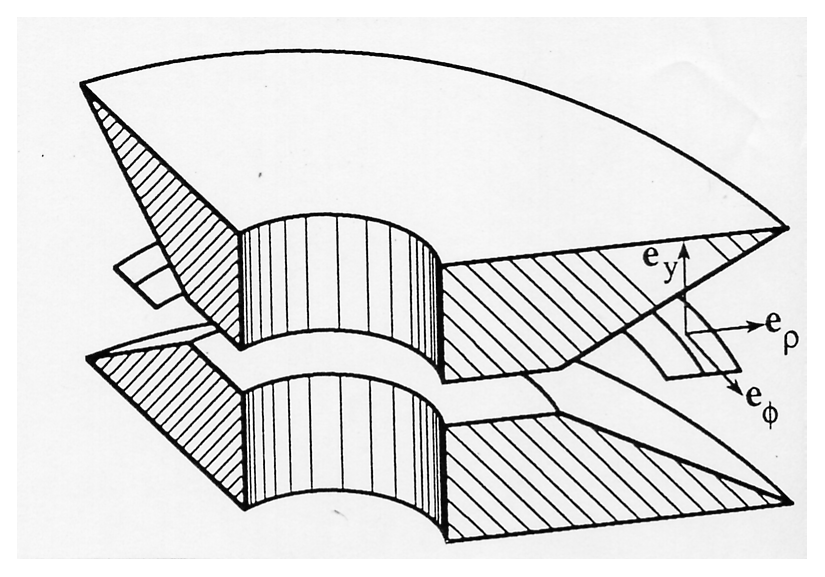
\includegraphics[height=3in]{dipole}
  \caption{Combined Function Dipole whose poles are surfaces of revolution.}
\end{figure}

%\newpage
\noindent where $B_0$ is the dipole strength.  Then it can be shown that the vector potential can be taken to have only a phi component with the expansion
\begin{equation}
\rho A_{\phi} = \sum_n U_n(\xi ,\eta ).
\end{equation}
Here
\begin{equation}
U_n = P_n + S_n
\end{equation}
with
\begin{equation}
U_0 = -\frac{B_0}{2} \rho^2_0,
\end{equation}
\begin{equation}
U_1 = -B_0\rho_0\xi ,
\end{equation}
\begin{equation}
P_2 = -\frac{B_0}{2} \xi^2 ,
\end{equation}
\begin{equation}
S_2 = -\frac{b_2\rho_0}{2}  (\xi^2 - \eta^2) + \frac{a_2\rho_0}{2} (2\xi \eta ),
\end{equation}
\begin{equation}
P_3 = -\frac{b_2}{8} \xi  (\xi^2 + \eta^2) + \frac{a_2}{8} \eta (\xi^2 + \eta^2),
\end{equation}
\begin{equation}
S_3 = -\frac{b_3\rho_0}{3}  (\xi^3 - 3\xi \eta^2) + \frac{a_3\rho_0}{3} (3\xi^2 \eta - \eta^3),
\end{equation}
\begin{equation}
P_4 = \frac{b_2}{64\rho_0}  (\xi^2 + \eta^2)^2 - \left( \frac{b_3}{12} - \frac{b_2}{32\rho_0}\right) (\xi^4 -\eta^4) + \left( \frac{a_3}{6} - \frac{a_2}{16\rho_0}\right) \xi \eta (\xi^2 + \eta^2),
\end{equation}
\begin{equation}
S_4 = -\frac{b_4\rho_0}{4}  (\xi^4 - 6\xi^2\eta^2 + \eta^4) + \frac{a_4\rho_0}{4} (4\xi^3\eta - 4\xi \eta^3), \ {\rm etc.}
\end{equation}


Correspondingly, the components of the magnetic field are given by the relations
\begin{eqnarray}
B_{\rho}(\xi,\eta) &= & \displaystyle \frac{1}{\rho} \frac{\partial}{\partial y} (\rho A_{\phi}) = \frac{1}{(\rho_0 + \xi )} \frac{\partial}{\partial \eta} (\rho A_{\phi}) \nonumber \\
&= & \displaystyle b_2 \eta +a_2\xi +\eta^2(-a_3 + \frac{3a_2}{8\rho_0})
+ \eta\xi(2b_3 - \frac{5b_2}{4\rho_0}) + \xi^2(a_3-\frac{7a_2}{8\rho_0}) \nonumber \\
& &\displaystyle + \eta^3(-b_4 - \frac{b_2}{16\rho_0^2} + \frac{b_3}{3\rho_0}) +\eta^2\xi(-3a_4 - \frac{9a_2}{16\rho_0^2} +\frac{3a_3}{2\rho_0})\nonumber \\
& &\displaystyle + \eta\xi^2(3b_4 + \frac{21b_2}{16\rho_0^2} - \frac{2b_3}{\rho_0})
+ \xi^3(a_4 + \frac{13a_2}{16\rho_0^2} - \frac{5a_3}{6\rho_0}),
\end{eqnarray}
\begin{eqnarray}
B_y(\xi,\eta) &= &\displaystyle -\frac{1}{\rho} \frac{\partial}{\partial \rho} (\rho A_{\phi}) = -\frac{1}{(\rho_0 + \xi)} \frac{\partial}{\partial \xi} (\rho A_{\phi}) \nonumber \\
&= &\displaystyle B_0-a_2\eta + b_2\xi + \eta^2(-b_3 + \frac{b_2}{8\rho_0}) + \eta\xi(-2a_3 + \frac{3a_2}{4\rho_0}) \nonumber \\
& &\displaystyle + \xi^2(b_3 - \frac{5b_2}{8\rho_0}) + \eta^3(
a_4 + \frac{a_2}{16\rho_0^2} - \frac{a_3}{6\rho_0}) + \eta^2\xi(
-3b_4 - \frac{3b_2}{16\rho_0^2} + \frac{b_3}{\rho_0}) \nonumber \\
& &\displaystyle + \eta\xi^2(-3a_4 - \frac{9a_2}{16\rho_0^2} + \frac{3a_3}{2\rho_0})
+\xi^3(b_4 + \frac{7b_2}{16\rho_0^2} - \frac{2b^3}{3\rho_0}),
\end{eqnarray}
\begin{equation}
B_{\phi} = 0.
\end{equation}
Here we have used the notation
\[
\begin{array}{lclclcl}
b_2&=&\mbox{BQD}&,&a_2&=&\mbox{AQD}\\
b_3&=&\mbox{BSEX}&,&a_3&=&\mbox{ASEX}\\
b_4&=&\mbox{BOCT}&,&a_4&=&\mbox{AOCT}.
\end{array} \]

For some applications it is convenient to specify the midplane field in terms of Taylor coefficients instead of the multipole coefficients $b_2$, $b_3$, and $b_4$.  Suppose the midplane vertical field is expanded in the Taylor form
     \begin{equation}
     B_y(\xi,0) = B_0 +t_1 \xi + t_2 \xi^2 + t_3 \xi^3 + \cdots.
     \end {equation}
%\pagebreak
Then, comparison with the results above gives the relations
\begin{equation}
t_1 = b_2,
\end{equation}
\begin{equation}
t_2 = b_3 - \frac{5b_2}{8\rho_0},
\end{equation}
\begin{equation}
t_3 = b_4 + \frac{7b_2}{16\rho_0^2} - \frac{2b_3}{3\rho_0},
\end{equation}
and the inverse relations
\begin{equation}
b_2 = t_1,
\end{equation}
\begin{equation}
b_3 =\frac{5t_1}{8\rho_0} + t_2,
\end{equation}
\begin{equation}
b_4 = -\frac{t_1}{48\rho_0^2} + \frac{2t_2}{3\rho_0} + t_3.
\end{equation}

Observe that if there is a nonzero quadrupole component ($b_2$ and/or $a_2 \neq 0$), then $U_3$ (and all the $U_n$ with $n >2$) cannot vanish.  Also if a sextupole component is nonzero, then all the $U_n$ with $n > 3$ cannot vanish.  This can be shown to be a simple consequence of Maxwell's equations when employed with curvilinear coordinates.  {\em The presence of multilpoles in curvilinear coordinates has a feed-up effect.}

The $U_n$ terms produce aberrations of order $(n-1)$.  It follows that if the combined function dipole we have been describing has nonzero gradient, then it must also produce second (and higher) order aberrations.  These aberrations will in general produce chromatic effects if the dispersion is nonzero.  Thus, for example, combined function dipoles generally affect the chromaticity of a ring in a complicated way.  The reader should be warned that not all accelerator design codes take this effect into account.  In particular, one cannot properly obtain the chromatic effects of a combined function dipole simply  by cutting an ordinary dipole into many segments and then inserting thin-lens quadrupoles (and/or higher order multipoles) between the segments.

For other applications (perhaps largely historical) it is convenient to specify the midplane field in terms of an {\em index} $n$ by making the Ansatz
\begin{equation}
B_y(\xi ,0) = B_0[\rho_0/(\rho_0 + \xi)]^n.
\end{equation}
In this case the Taylor coefficients are given by the relations
\begin{equation}
t_1 = -nB_0/\rho_0,
\end{equation}
\begin{equation}
t_2 = n(n+1) B_0/(2\rho_0^2),
\end{equation}
\begin{equation}
t_3 = -n(n+1)(n+2) B_0/(6\rho_0^3).
\end{equation}
\index{index} \index{field index}

     The true fringe fields of a combined function dipole are also a very
complicated affair.  Correspondingly, their proper treatment requires the
use of GENMAP (see section 1.4.1) or equivalent routines based upon field data obtained either from high accuracy 3-dimensional magnet code calculations (such calculations are near the current state of the art) or very careful field measurements.  In the absence of such heroic efforts, one may estimate the effect of fringe fields by using the current \Mary hard-edge models for dipoles and quadrupoles.  That is, an approximation to the full transfer map for the combined function dipole in the hard-edge limit can be obtained simply by pre- and post-multiplying the transfer maps of pure dipoles and pure quadrupoles having strengths corresponding to those associated with the combined function dipole parameters.  This option, or the option of supplying one's own fringe-field transfer maps, is controlled by the parameters LFRN and TFRN.

Where the \Mary hard-edge model is used for the dipole portion of the fringe field, the gap size and normalized field integral are given default values of 0 and .5, respectively.  If other values are desired, they may be set using a command with the type code
{\em cfrn}.  See section 6.29.

For further detail, see references listed in Chapter 11.


\clearpage

\begin{footnotesize}
\begin{verbatim}
#comment
 Exhibit 6.8.1.
 This is a MARYLIE run illustrating the sign conventions for
 combined function bends.  A combined function bend is a bend
 with added quadrupole, sextupole, and octupole components.
 Thus, pure dipoles, pure quadrupoles, pure sextupoles,
 and pure octupoles are special cases of the combined function
 bend.  This is verified below for various cases.  Note that to
 obtain a finite length element without dipole content using
 the cfbd element, it is necessary to make both the dipole field
 small and the bend angle small in such a way that the design orbit
 path length as given in figure 6.2a takes on the desired value.
 This limiting operation is not necessary, of course, since
 there are special type codes for this purpose.  However, it
 is done here to illustrate that the combined function bend
 does have the right limiting behavior.
 For simplicity of calculation the value of brho has been set
 equal to 10/pi.  Thus, the path length is given by the relation

  path length = 10/180 * theta (in degrees) /B.

 In particular, if

      theta = 9.e-9 and B = 1.e-9,
 then

       path length = .5 meters.

#beam
  3.183098861830000
 0.8526309382400936
  1.000000000000000
  1.000000000000000
#menu
 fileout  pmif
   1.00000000000000       12.0000000000000       3.00000000000000
 setzero  zer
  0.000000000000000E+00  1.000000000000000E-08  0.000000000000000E+00
 mapout   ptm
   3.00000000000000       3.00000000000000      0.000000000000000E+00
  0.000000000000000E+00   1.00000000000000
 cfbd36   cfbd
   36.0000000000000       1.20000000000000       1.00000000000000
   1.00000000000000       1.00000000000000       1.00000000000000
 wcfbd    cfbd
  9.000000000000000E-09  1.000000000000000E-09   1.00000000000000
   1.00000000000000       1.00000000000000       1.00000000000000
 bpar     ps1
  0.000000000000000E+00  0.000000000000000E+00  0.000000000000000E+00
  0.000000000000000E+00  0.000000000000000E+00  0.000000000000000E+00
 qpar     ps1
   5.00000000000000      0.000000000000000E+00  0.000000000000000E+00
  0.000000000000000E+00  0.000000000000000E+00  0.000000000000000E+00
 skqpar   ps1
  0.000000000000000E+00   5.00000000000000      0.000000000000000E+00
  0.000000000000000E+00  0.000000000000000E+00  0.000000000000000E+00
 spar     ps1
  0.000000000000000E+00  0.000000000000000E+00   20.0000000000000
  0.000000000000000E+00  0.000000000000000E+00  0.000000000000000E+00
 skspar   ps1
  0.000000000000000E+00  0.000000000000000E+00  0.000000000000000E+00
   20.0000000000000      0.000000000000000E+00  0.000000000000000E+00
 opar     ps1
  0.000000000000000E+00  0.000000000000000E+00  0.000000000000000E+00
  0.000000000000000E+00   20.0000000000000      0.000000000000000E+00
 skopar   ps1
  0.000000000000000E+00  0.000000000000000E+00  0.000000000000000E+00
  0.000000000000000E+00  0.000000000000000E+00   20.0000000000000
 nbnd     nbnd
   36.0000000000000      0.000000000000000E+00  0.500000000000000
   1.20000000000000       1.00000000000000       1.00000000000000
 hfqd     quad
  0.500000000000000       5.00000000000000       1.00000000000000
   1.00000000000000
 sex      sext
  0.500000000000000       20.0000000000000
 oct      octm
  0.500000000000000       20.0000000000000
 arot+q   arot
   45.0000000000000
 arot-q   arot
  -45.0000000000000
 arot+s   arot
   30.0000000000000
 arot-s   arot
  -30.0000000000000
 arot+o   arot
   22.5000000000000
 arot-o   arot
  -22.5000000000000
 clear    iden
 inv      inv
 end      end
#lines
 pcfbd
     1*bpar        1*cfbd36
 qcfbd
     1*qpar        1*wcfbd
 skqcfbd
     1*skqpar      1*wcfbd
 scfbd
     1*spar        1*wcfbd
 skscfbd
     1*skspar      1*wcfbd
 ocfbd
     1*opar        1*wcfbd
 skocfbd
     1*skopar      1*wcfbd
 skquad
     1*arot+q      1*hfqd        1*arot-q
 sksex
     1*arot+s      1*sex         1*arot-s
 skoct
     1*arot+o      1*oct         1*arot-o
 bendtest
     1*clear       1*nbnd        1*inv         1*pcfbd       1*mapout
 quadtest
     1*clear       1*hfqd        1*inv         1*qcfbd       1*mapout   &
     1*clear       1*skquad      1*inv         1*skqcfbd     1*mapout
 sextest
     1*clear       1*sex         1*inv         1*scfbd       1*mapout   &
     1*clear       1*sksex       1*inv         1*skscfbd     1*mapout
 octtest
     1*clear       1*oct         1*inv         1*ocfbd       1*mapout   &
     1*clear       1*skoct       1*inv         1*skocfbd     1*mapout
#lumps
#loops
#labor
    1*fileout
    1*setzero
    1*bendtest
    1*quadtest
    1*sextest
    1*octtest
    1*end
\end{verbatim}
\end{footnotesize}
Result of bendtest
\begin{footnotesize}
\begin{verbatim}
matrix for map is :

 1.00000E+00  3.88578E-16  0.00000E+00 -2.77556E-17  0.00000E+00 -1.52656E-16
-2.42861E-17  1.00000E+00  1.73472E-18 -2.89121E-18  0.00000E+00 -5.82867E-16
-6.15035E-18 -2.24547E-17  1.00000E+00  2.77556E-17  0.00000E+00 -1.93800E-17
 1.40342E-18 -2.70469E-18  0.00000E+00  1.00000E+00  0.00000E+00 -1.04395E-18
-2.91434E-16  2.35922E-16  0.00000E+00  0.00000E+00  1.00000E+00  8.32667E-17
 0.00000E+00  0.00000E+00  0.00000E+00  0.00000E+00  0.00000E+00  1.00000E+00

nonzero elements in generating polynomial are :

\end{verbatim}
\end{footnotesize}
Result of quadtest
\begin{footnotesize}
\begin{verbatim}
matrix for map is :

 1.00000E+00 -1.24191E-12  3.33861E-17 -1.48041E-17  0.00000E+00 -4.51426E-11
 1.95068E-12  1.00000E+00 -2.32542E-17  3.33861E-17  0.00000E+00 -1.74622E-10
 1.12409E-17 -6.49358E-18  1.00000E+00 -1.24187E-12  0.00000E+00 -4.03897E-28
 1.58205E-17  7.99411E-18 -1.95086E-12  1.00000E+00  0.00000E+00  0.00000E+00
 1.74622E-10 -4.51426E-11  0.00000E+00  0.00000E+00  1.00000E+00 -5.10553E-13
 0.00000E+00  0.00000E+00  0.00000E+00  0.00000E+00  0.00000E+00  1.00000E+00

nonzero elements in generating polynomial are :


matrix for map is :

 1.00000E+00 -1.24187E-12 -2.41506E-17  1.90820E-17  0.00000E+00 -4.66693E-11
-2.42861E-17  1.00000E+00 -1.95080E-12  1.04083E-17  0.00000E+00 -1.86837E-10
-3.46945E-17  2.42861E-17  1.00000E+00 -1.24188E-12  0.00000E+00 -1.52674E-12
-1.95087E-12  2.42861E-17  1.73472E-17  1.00000E+00  0.00000E+00 -1.22150E-11
 1.86837E-10 -4.66693E-11  1.22150E-11 -1.52674E-12  1.00000E+00 -5.10553E-13
 0.00000E+00  0.00000E+00  0.00000E+00  0.00000E+00  0.00000E+00  1.00000E+00

nonzero elements in generating polynomial are :

\end{verbatim}
\end{footnotesize}
Result of sextest
\begin{footnotesize}
\begin{verbatim}
matrix for map is :

 1.00000E+00 -1.24179E-12  0.00000E+00  0.00000E+00  0.00000E+00 -4.66493E-11
-4.93480E-20  1.00000E+00  0.00000E+00  0.00000E+00  0.00000E+00 -1.86597E-10
 0.00000E+00  0.00000E+00  1.00000E+00 -1.24179E-12  0.00000E+00  4.03897E-28
 0.00000E+00  0.00000E+00  0.00000E+00  1.00000E+00  0.00000E+00 -3.23117E-27
 1.86597E-10 -4.66493E-11  3.23117E-27 -1.61559E-27  1.00000E+00 -5.10553E-13
 0.00000E+00  0.00000E+00  0.00000E+00  0.00000E+00  0.00000E+00  1.00000E+00

nonzero elements in generating polynomial are :


matrix for map is :

 1.00000E+00 -1.24179E-12  0.00000E+00  0.00000E+00  0.00000E+00 -4.66493E-11
-4.93480E-20  1.00000E+00  0.00000E+00  0.00000E+00  0.00000E+00 -1.86597E-10
 0.00000E+00  0.00000E+00  1.00000E+00 -1.24179E-12  0.00000E+00  4.03897E-28
 0.00000E+00  0.00000E+00  0.00000E+00  1.00000E+00  0.00000E+00 -3.23117E-27
 1.86597E-10 -4.66493E-11  3.23117E-27 -1.61559E-27  1.00000E+00 -5.10553E-13
 0.00000E+00  0.00000E+00  0.00000E+00  0.00000E+00  0.00000E+00  1.00000E+00

nonzero elements in generating polynomial are :

\end{verbatim}
\end{footnotesize}
Result of octtest
\begin{footnotesize}
\begin{verbatim}
matrix for map is :

 1.00000E+00 -1.24179E-12  0.00000E+00  0.00000E+00  0.00000E+00 -4.66493E-11
-4.93480E-20  1.00000E+00  0.00000E+00  0.00000E+00  0.00000E+00 -1.86597E-10
 0.00000E+00  0.00000E+00  1.00000E+00 -1.24179E-12  0.00000E+00  4.03897E-28
 0.00000E+00  0.00000E+00  0.00000E+00  1.00000E+00  0.00000E+00 -3.23117E-27
 1.86597E-10 -4.66493E-11  3.23117E-27 -1.61559E-27  1.00000E+00 -5.10553E-13
 0.00000E+00  0.00000E+00  0.00000E+00  0.00000E+00  0.00000E+00  1.00000E+00

nonzero elements in generating polynomial are :


matrix for map is :

 1.00000E+00 -1.24179E-12  0.00000E+00  0.00000E+00  0.00000E+00 -4.66493E-11
-4.93480E-20  1.00000E+00  0.00000E+00  0.00000E+00  0.00000E+00 -1.86597E-10
 0.00000E+00  0.00000E+00  1.00000E+00 -1.24179E-12  0.00000E+00  4.03897E-28
 0.00000E+00  0.00000E+00  0.00000E+00  1.00000E+00  0.00000E+00 -3.23117E-27
 1.86597E-10 -4.66493E-11  3.23117E-27 -1.61559E-27  1.00000E+00 -5.10553E-13
 0.00000E+00  0.00000E+00  0.00000E+00  0.00000E+00  0.00000E+00  1.00000E+00

nonzero elements in generating polynomial are :
\end{verbatim}
\end{footnotesize}

\newpage
\section{Magnetic Quadrupole}
\begin{quotation}
\noindent Type Code:  quad
\vspace{5mm}

\noindent Required Parameters:
\begin{enumerate}
      \item  Length of quadrupole (m).

      \item  Strength, $Q$ (Tesla/m).

             When $Q > 0$, the quadrupole is horizontally focusing.

             When $Q < 0$, the quadrupole is horizontally defocusing.

      \item  LFRN

             \ = 0 for no fringe field on leading edge (entry) of quadrupole.

             \ = 1 for hard-edge fringe field on leading edge of  quadrupole.

      \item  TFRN

             \ = 0 for no fringe field on trailing edge (exit) of quadrupole.

             \ = 1 for hard-edge fringe field on trailing edge of quadrupole.
\end{enumerate}

\vspace{5mm}
\noindent Example:
\begin{verbatim}
         hfq    quad
          .5  , 1.92, 1, 1
\end{verbatim}
\end{quotation}
This specifies a quadrupole with the user given name {\em hfq}.\index{quadrupole}  It has a length
of .5 meters, a strength of 1.92 Tesla/meter, is horizontally focusing, and
has hard-edge leading and trailing fringe fields.

\vspace{5mm}
     Vector Potential:  $\displaystyle A_z = -\frac{Q}{2}(x^2-y^2)$

\vspace{5mm}
     Remark:
\vspace{2mm}

         There is no type code for the quadrupole hard-edge fringe field
transfer maps by themselves.  However, they may be obtained from the
quadrupole transfer map by setting the length equal to zero.

\vspace{5mm}
\begin{quotation}
\noindent Example:
\begin{verbatim}
         lqff    quad
          0 ,  1.92 ,  1 ,  0
\end{verbatim}
\end{quotation}
This specifies a map with the user given name {\em lqff}.  It is the map for the
\underline leading \underline quadrupole \underline fringe \underline field of a quadrupole having a strength of 1.92 Tesla/meter.

\pagebreak

\vspace{5mm}
     Description:
\vspace{2mm}

\nopagebreak
     From the relation ${\bf B} = \nabla \times {\bf A}$ one has the result
\begin{eqnarray*}
B_x &=& \partial_y A_z - \partial_z A_y = Qy,\\
B_y &=& \partial_z A_x - \partial_x A_z = Qx,\\
B_z &=& \partial_x A_y - \partial_y A_x = 0.
\end{eqnarray*}
See figure 6.9.1 for a plot of the midplane vertical field $B_y$ for the horizontally focusing case $Q>0$.

   Note that one has the relations
\[ \|{\bf B}\|^2 = B_x^2 + B_y^2 = Q^2 y^2 + Q^2 x^2 = Q^2 r^2.\]
See figure 6.9.2.  It follows that if $B$ is the pole tip magnetic field and $R$ is the pole tip radius, then the quadrupole strength $Q$ is given by the relation
\[Q=\frac{B}{R}.\]

   The map for a quadrupole rotated clockwise by angle $\theta$ about the
   $z$-axis may be gotten by preceding and following the map for a
   regular quadrupole by maps corresponding to {\em arot\/}$(-\theta)$ and {\em arot\/}$(+\theta)$, respectively.  See Exhibit 6.9.1 and figure 6.14.3.

   Suppose the vector potential for a rotated quadrupole is written in the form
\[ A_z = -\frac{b}{2}(x^2-y^2) + \frac{a}{2}2xy. \]
Here $b$ and $a$ are by definition the normal and skew components of the
quadrupole strength.  Correspondingly, from ${\bf B} = \nabla \times
{\bf A}$, the components of the magnetic field are given by the relations

\[\begin{array}{cl}
B_x=ax+by,&(*)\\
B_y=bx-ay,&(**)\\
B_z =0.
\end{array}\]
Note that the relations $(*)$ and $(**)$ are equivalent to the formal complex relation
\[ B_y + iB_x = (b+ia)(x+iy). \]
Then, with these definitions, the quantities $a, b, Q, \mbox{and } \theta$ are connected by the relations
\begin{eqnarray*}
a&=&-Q\sin(2\theta) ,\\
b&=&Q\cos(2\theta).
\end{eqnarray*}
Thus, what is usually called a ``positive'' skew quadrupole is gotten by
rotating a normal quadrupole by $-45^\circ$ around the $z$-axis.
Correspondingly, the poles for a positive skew quadrupole are configured as shown in figure 6.9.3.  For this quadrupole the magnetic field is given by the relations
\[ B_x=ax,B_y=-ay,B_z=0, \]
with $a=Q$.


\begin{figure}
  \centering
  \includegraphics[scale=0.453]{MagneticFieldQuad}
  \caption{Midplane magnetic field of a normal quadrupole that horizontally focuses positive particles (end view).
Particles on the design orbit move in the $+z$ direction along the $z$
axis.}
\end{figure}

\begin{figure}
  \centering
  \includegraphics[scale=0.453]{QuadConfig}
  \caption{Pole configuration for the quadrupole of figure 6.9.1, same end view.}
\end{figure}

\begin{figure}
  \centering
  \includegraphics[scale=0.453]{QuadSkewConfig}
  \caption{Pole configuration for a positive skew quadrupole, end view.
Note that this figure is gotten by rotating the poles in figure 6.9.2 by $-45^\circ$ clockwise.  That is, the rotation is $+45^\circ$ counterclockwise.}
\end{figure}

\clearpage


\begin{footnotesize}
\begin{verbatim}
#comment
 Exhibit 6.9.1.
 This is a MARYLIE run illustrating the sign conventions for a
 a quadrupole.  First, it is shown that for positive particles a quadrupole with positive
 strength is horizontally focusing and vertically defocusing.
 Next, the map for a quadrupole "rotquad" rotated clockwise by angle
 theta about the z axis is gotten by the rule

    rotquad = arot(-theta) * quad * arot(theta).

 Also, what is usually called a skew quad is the result of setting
 theta = -45 degrees.  Thus, the map "skewquad" for a skew quad is
 gotten by the rule

    skewquad = arot(45) * quad * arot(-45).

 The beam parameters are those for 800 MeV protons.
#beam
  4.881030646470486
 0.8526309382400936
  1.000000000000000
  1.000000000000000
#menu
 fileout  pmif
   1.00000000000000       12.0000000000000       3.00000000000000
 matout   ptm
   3.00000000000000      0.000000000000000E+00  0.000000000000000E+00
  0.000000000000000E+00   1.00000000000000
 raysin   rt
   13.0000000000000       14.0000000000000      -1.00000000000000
  0.000000000000000E+00  0.000000000000000E+00  0.000000000000000E+00
 trace    rt
  0.000000000000000E+00   14.0000000000000       4.00000000000000
  0.000000000000000E+00   1.00000000000000      0.000000000000000E+00
 hfquad   quad
   1.00000000000000       3.00000000000000       1.00000000000000
   1.00000000000000
 arot+45  arot
   45.0000000000000
 arot-45  arot
  -45.0000000000000
 clear    iden
 end      end
#lines
 skewquad
     1*arot+45     1*hfquad      1*arot-45
#lumps
#loops
#labor
    1*fileout
    1*hfquad
    1*matout
    1*raysin
    1*trace
    1*clear
    1*skewquad
    1*matout
    1*trace
    1*end

matrix for map is :

 7.08109E-01  9.00665E-01  0.00000E+00  0.00000E+00  0.00000E+00  0.00000E+00
-5.53571E-01  7.08109E-01  0.00000E+00  0.00000E+00  0.00000E+00  0.00000E+00
 0.00000E+00  0.00000E+00  1.32338E+00  1.10563E+00  0.00000E+00  0.00000E+00
 0.00000E+00  0.00000E+00  6.79548E-01  1.32338E+00  0.00000E+00  0.00000E+00
 0.00000E+00  0.00000E+00  0.00000E+00  0.00000E+00  1.00000E+00  4.11143E-01
 0.00000E+00  0.00000E+00  0.00000E+00  0.00000E+00  0.00000E+00  1.00000E+00

matrix for map is :

 1.01574E+00  1.00315E+00  3.07635E-01  1.02483E-01  0.00000E+00  0.00000E+00
 6.29888E-02  1.01574E+00  6.16559E-01  3.07635E-01  0.00000E+00  0.00000E+00
 3.07635E-01  1.02483E-01  1.01574E+00  1.00315E+00  0.00000E+00  0.00000E+00
 6.16559E-01  3.07635E-01  6.29888E-02  1.01574E+00  0.00000E+00  0.00000E+00
 0.00000E+00  0.00000E+00  0.00000E+00  0.00000E+00  1.00000E+00  4.11143E-01
 0.00000E+00  0.00000E+00  0.00000E+00  0.00000E+00  0.00000E+00  1.00000E+00
\end{verbatim}
\end{footnotesize}
Initial conditions for ray traces (contents of file 13):
\begin{footnotesize}
\begin{verbatim}
 .01 .00 .00 .00 .00 .00
 .00 .00 .01 .00 .00 .00
\end{verbatim}
\end{footnotesize}
Final conditions for ray traces (contents of file 14):
\vspace{5mm}

\noindent Results for normal quadrupole
\begin{footnotesize}
\begin{verbatim}
 7.08109E-03 -5.53577E-03  0.00000E+00  0.00000E+00  6.61182E-06  0.00000E+00
 0.00000E+00  0.00000E+00  1.32339E-02  6.79527E-03  8.45425E-06  0.00000E+00
\end{verbatim}
\end{footnotesize}
Note that the first particle is focused horizontally, and the second is
defocused vertically.
\vspace{5mm}

\noindent Results for skew quadrupole
\begin{footnotesize}
\begin{verbatim}
 1.01574E-02  6.29633E-04  3.07638E-03  6.16559E-03  7.53303E-06  0.00000E+00
 3.07638E-03  6.16559E-03  1.01574E-02  6.29633E-04  7.53303E-06  0.00000E+00
\end{verbatim}
\end{footnotesize}
Note that the first particle is deflected in the $+y$ direction, and the
second particle is deflected in the $+x$ direction.


\newpage
\section{Magnetic Sextupole}
\begin{quotation}
\noindent Type Code:  sext
\vspace{5mm}

\noindent Required Parameters:
\begin{enumerate}
      \item  Length of sextupole (m).
      \item  Strength, $S$ (Tesla/$\mbox{m}^2$).  Consider a positive
particle passing through a sextupole and having an energy
             slightly larger than the design energy.  When $S > 0$ (and
             assuming the local eta dispersion function is positive), the
             sextupole provides horizontal focusing and vertical defocusing
             for such a particle.  It thus raises the horizontal
             chromaticity and lowers the vertical chromaticity.  When $S < 0$,
             the sextupole lowers the horizontal chromaticity and raises
             the vertical chromaticity.
\end{enumerate}

\vspace{5mm}
\noindent     Example:
\begin{verbatim}
         hcs    sext
         .5  ,  3.5
\end{verbatim}
\end{quotation}
This specifies a sextupole with the user given name {\em hcs}.\index{sextupole}  It has a length
of .5 meters and a strength of 3.5 Tesla/$\mbox{(meter)}^2$.  Under
normal usage it raises the
horizontal chromaticity and lowers the vertical chromaticity.

\vspace{5mm}
   Vector Potential:  $\displaystyle A_z  = - \frac{S}{3}(x^3 - 3xy^2)$

\vspace{5mm}
     Description:
\vspace{2mm}

    From the relation ${\bf B} = \nabla \times {\bf A}$ one has the result
\begin{eqnarray*}
B_x= & \partial_y A_z - \partial_z A_y &= 2Sxy,\\
B_y= & \partial_z A_x - \partial_x A_z &= S(x^2-y^2),\\
B_z= & \partial_x A_y - \partial_y A_x &= 0.
\end{eqnarray*}
See figure 6.10.1 for a plot of the midplane vertical field $B_y$ for the case $S>0$.

   Note that one has the relations
\begin{eqnarray*}
\|{\bf B}\|^2 &= B_x^2 + B_y^2 = 4S^2 x^2 y^2 + S^2(x^4-2x^2 y^2 + y^4)\\
&=S^2(x^4 + 2x^2 y^2 + y^4) = S^2 r^4.
\end{eqnarray*}
See figure 6.10.2.  It follows that if $B$ is the pole tip magnetic field and $R$ is the pole tip radius, then the sextupole strength $S$ is given by the relation
\[S=\frac{B}{R^2}.\]

   The map for a sextupole rotated clockwise by angle $\theta$ about the
   $z$-axis may be gotten by preceding and following the map for a
   regular sextupole by maps corresponding to {\em arot}$(-\theta)$ and {\em arot}$(+\theta)$, respectively.  See Exhibit 6.10.1 and figure 6.14.3.

   Suppose the vector potential for a rotated sextupole is written in the form
\[A_z = -\frac{b}{3}(x^3 - 3xy^2) + \frac{a}{3}(3x^2 y - y^3). \]
Here $b$ and $a$ are by definition the normal and skew components of the
sextupole strength.  Correspondingly, from ${\bf B} = \nabla \times
{\bf A}$, the components of the magnetic field are given by the relations
\[\begin{array}{cl}
B_x=2bxy+a(x^2 - y^2),&(*)\\
B_y=b(x^2-y^2)-2axy,&(**)\\
B_z =0.
\end{array}\]
Note that the relations (*) and (**) are equivalent to the formal complex relation
\[B_y + iB_x = (b+ia)(x + iy)^2.\]
Then, with these definitions, the quantities $a$, $b$, $S$, and $\theta$ are connected by the relations
\begin{eqnarray*}
a&=&-S\sin(3\theta) ,\\
b&=&S\cos(3\theta).
\end{eqnarray*}
Thus, what is usually called a ``positive'' skew sextupole is gotten by
rotating a normal sextupole by $-30^\circ$ around the $z$-axis.
Correspondingly, the poles for a positive skew sextupole are configured as shown in figure 6.10.3.  For this sextupole the magnetic field is given by the relations
\[B_x = a(x^2 - y^2) , B_y = -2axy , B_z = 0, \]
with $a=S$.


\begin{figure}[hp]
  \centering
  \includegraphics[scale=0.453]{MagneticFieldSext}
  \caption{End view showing midplane magnetic field of a normal
sextupole that provides horizontal focusing for a positive particle if
$x > 0$ and horizontal defocusing if $x < 0$.  Note that such a sextupole
always provides (for a positive particle) a net deflection in the $-x$
direction unless x is initially zero.  See Exhibit 6.10.1.}
\end{figure}


\begin{figure}[hp]
  \centering
  \includegraphics[scale=0.453]{SextConfig}
  \caption{Pole configuration for the sextupole of figure 6.10.1, same end view.}
\end{figure}


\begin{figure}[hp]
  \centering
  \includegraphics[scale=0.453]{SextSkewConfig}
  \caption{Pole configuration for a positive skew sextupole, end view.
Note that this figure is gotten by rotating the poles in figure 6.10.2 by $-30^{\circ}$ clockwise.  That is, the rotation is $+30^\circ$ counterclockwise.}
\end{figure}

\clearpage
\begin{footnotesize}
\begin{verbatim}
#comment
 Exhibit 6.10.1.
 This is a MARYLIE run illustrating the sign conventions for a
 a sextupole.  First, it is shown that a sextupole always deflects a
 positive particle
 in the -x direction unless x is initially zero.
 Next, the map for a sextupole "rotsext" rotated clockwise by angle
 theta about the z axis is gotten by the rule

    rotsext = arot(-theta) * sext * arot(theta).

 Also, what is usually called a positive skew sextupole is the result
 of setting theta = -30 degrees.  Thus, the map "skewsext" for a skew
 sextupole is gotten by the rule

    skewsext = arot(30) * sext * arot(-30).

 The beam parameters are those for 800 MeV protons.
#beam
  4.881030646470486
 0.8526309382400936
  1.000000000000000
  1.000000000000000
#menu
 fileout  pmif
   1.00000000000000       12.0000000000000       3.00000000000000
 setzero  czer
  1.000000000000000E-14  0.000000000000000E+00
 mapout   ptm
   3.00000000000000       3.00000000000000      0.000000000000000E+00
  0.000000000000000E+00   1.00000000000000
 raysin   rt
   13.0000000000000       14.0000000000000      -1.00000000000000
  0.000000000000000E+00  0.000000000000000E+00  0.000000000000000E+00
 trace    rt
  0.000000000000000E+00   14.0000000000000       4.00000000000000
  0.000000000000000E+00   1.00000000000000      0.000000000000000E+00
 sext     sext
  0.500000000000000       3.00000000000000
 arot+30  arot
   30.0000000000000
 arot-30  arot
  -30.0000000000000
 clear    iden
 end      end
#lines
 skewsext
     1*arot+30     1*sext        1*arot-30
#lumps
#loops
#labor
    1*fileout
    1*setzero
    1*sext
    1*mapout
    1*raysin
    1*trace
    1*clear
    1*skewsext
    1*mapout
    1*trace
    1*end

matrix for map is :

 1.00000E+00  5.00000E-01  0.00000E+00  0.00000E+00  0.00000E+00  0.00000E+00
 0.00000E+00  1.00000E+00  0.00000E+00  0.00000E+00  0.00000E+00  0.00000E+00
 0.00000E+00  0.00000E+00  1.00000E+00  5.00000E-01  0.00000E+00  0.00000E+00
 0.00000E+00  0.00000E+00  0.00000E+00  1.00000E+00  0.00000E+00  0.00000E+00
 0.00000E+00  0.00000E+00  0.00000E+00  0.00000E+00  1.00000E+00  2.05572E-01
 0.00000E+00  0.00000E+00  0.00000E+00  0.00000E+00  0.00000E+00  1.00000E+00

nonzero elements in generating polynomial are :

 f( 28)=f( 30 00 00 )=-0.10243738181844D+00
 f( 29)=f( 21 00 00 )= 0.76828036363829D-01
 f( 34)=f( 12 00 00 )=-0.25609345454610D-01
 f( 39)=f( 10 20 00 )= 0.30731214545532D+00
 f( 40)=f( 10 11 00 )=-0.15365607272766D+00
 f( 43)=f( 10 02 00 )= 0.25609345454610D-01
 f( 49)=f( 03 00 00 )= 0.32011681818262D-02
 f( 53)=f( 02 00 01 )=-0.29697889251752D+00
 f( 54)=f( 01 20 00 )=-0.76828036363829D-01
 f( 55)=f( 01 11 00 )= 0.51218690909220D-01
 f( 58)=f( 01 02 00 )=-0.96035045454787D-02
 f( 76)=f( 00 02 01 )=-0.29697889251752D+00
 f( 83)=f( 00 00 03 )=-0.12210091207749D+00
 f( 84)=f( 40 00 00 )= 0.39350314476813D-02
 f( 85)=f( 31 00 00 )=-0.39350314476813D-02
 f( 90)=f( 22 00 00 )= 0.14756367928805D-02
 f( 95)=f( 20 20 00 )= 0.78700628953625D-02
 f( 96)=f( 20 11 00 )=-0.39350314476813D-02
 f( 99)=f( 20 02 00 )= 0.98375786192031D-04
 f(105)=f( 13 00 00 )=-0.24593946548008D-03
 f(109)=f( 12 00 01 )=-0.15210870102417D-01
 f(110)=f( 11 20 00 )=-0.39350314476813D-02
 f(111)=f( 11 11 00 )= 0.27545220133769D-02
 f(114)=f( 11 02 00 )=-0.24593946548008D-03
 f(132)=f( 10 02 01 )= 0.15210870102417D-01
 f(140)=f( 04 00 00 )=-0.62482432895323D-01
 f(144)=f( 03 00 01 )= 0.38027175256043D-02
 f(145)=f( 02 20 00 )= 0.98375786192031D-04
 f(146)=f( 02 11 00 )=-0.24593946548008D-03
 f(149)=f( 02 02 00 )=-0.12496486579065D+00
 f(154)=f( 02 00 02 )=-0.40417877560560D+00
 f(161)=f( 01 11 01 )= 0.30421740204834D-01
 f(167)=f( 01 02 01 )=-0.11408152576813D-01
 f(175)=f( 00 40 00 )= 0.39350314476813D-02
 f(176)=f( 00 31 00 )=-0.39350314476813D-02
 f(179)=f( 00 22 00 )= 0.14756367928805D-02
 f(185)=f( 00 13 00 )=-0.24593946548008D-03
 f(195)=f( 00 04 00 )=-0.62482432895323D-01
 f(200)=f( 00 02 02 )=-0.40417877560560D+00
 f(209)=f( 00 00 04 )=-0.15561050561982D+00

matrix for map is :

 1.00000E+00  5.00000E-01  0.00000E+00  0.00000E+00  0.00000E+00  0.00000E+00
 0.00000E+00  1.00000E+00  0.00000E+00  0.00000E+00  0.00000E+00  0.00000E+00
 0.00000E+00  0.00000E+00  1.00000E+00  5.00000E-01  0.00000E+00  0.00000E+00
 0.00000E+00  0.00000E+00  0.00000E+00  1.00000E+00  0.00000E+00  0.00000E+00
 0.00000E+00  0.00000E+00  0.00000E+00  0.00000E+00  1.00000E+00  2.05572E-01
 0.00000E+00  0.00000E+00  0.00000E+00  0.00000E+00  0.00000E+00  1.00000E+00

nonzero elements in generating polynomial are :

 f( 30)=f( 20 10 00 )= 0.30731214545532D+00
 f( 31)=f( 20 01 00 )=-0.76828036363829D-01
 f( 35)=f( 11 10 00 )=-0.15365607272766D+00
 f( 36)=f( 11 01 00 )= 0.51218690909220D-01
 f( 50)=f( 02 10 00 )= 0.25609345454610D-01
 f( 51)=f( 02 01 00 )=-0.96035045454787D-02
 f( 53)=f( 02 00 01 )=-0.29697889251752D+00
 f( 64)=f( 00 30 00 )=-0.10243738181844D+00
 f( 65)=f( 00 21 00 )= 0.76828036363829D-01
 f( 68)=f( 00 12 00 )=-0.25609345454610D-01
 f( 74)=f( 00 03 00 )= 0.32011681818262D-02
 f( 76)=f( 00 02 01 )=-0.29697889251752D+00
 f( 83)=f( 00 00 03 )=-0.12210091207749D+00
 f( 84)=f( 40 00 00 )= 0.39350314476813D-02
 f( 85)=f( 31 00 00 )=-0.39350314476813D-02
 f( 90)=f( 22 00 00 )= 0.14756367928805D-02
 f( 95)=f( 20 20 00 )= 0.78700628953625D-02
 f( 96)=f( 20 11 00 )=-0.39350314476813D-02
 f( 99)=f( 20 02 00 )= 0.98375786192031D-04
 f(105)=f( 13 00 00 )=-0.24593946548008D-03
 f(110)=f( 11 20 00 )=-0.39350314476813D-02
 f(111)=f( 11 11 00 )= 0.27545220133769D-02
 f(114)=f( 11 02 00 )=-0.24593946548008D-03
 f(116)=f( 11 01 01 )= 0.30421740204834D-01
 f(140)=f( 04 00 00 )=-0.62482432895323D-01
 f(145)=f( 02 20 00 )= 0.98375786192031D-04
 f(146)=f( 02 11 00 )=-0.24593946548008D-03
 f(148)=f( 02 10 01 )= 0.15210870102417D-01
 f(149)=f( 02 02 00 )=-0.12496486579065D+00
 f(151)=f( 02 01 01 )=-0.11408152576813D-01
 f(154)=f( 02 00 02 )=-0.40417877560560D+00
 f(175)=f( 00 40 00 )= 0.39350314476813D-02
 f(176)=f( 00 31 00 )=-0.39350314476813D-02
 f(179)=f( 00 22 00 )= 0.14756367928805D-02
 f(185)=f( 00 13 00 )=-0.24593946548008D-03
 f(187)=f( 00 12 01 )=-0.15210870102417D-01
 f(195)=f( 00 04 00 )=-0.62482432895323D-01
 f(197)=f( 00 03 01 )= 0.38027175256043D-02
 f(200)=f( 00 02 02 )=-0.40417877560560D+00
 f(209)=f( 00 00 04 )=-0.15561050561982D+00
\end{verbatim}
\end{footnotesize}
Initial conditions for ray traces (contents of file 13):
\begin{footnotesize}
\begin{verbatim}
-.01 .00 .00 .00 .00 .00
+.01 .00 .00 .00 .00 .00
\end{verbatim}
\end{footnotesize}
Final conditions for ray traces (contents of file 14):
\vspace{5mm}

\noindent Results for normal sextupole
\begin{footnotesize}
\begin{verbatim}
-1.00077E-02 -3.07470E-05  0.00000E+00  0.00000E+00  9.34897E-11  0.00000E+00
 9.99232E-03 -3.07155E-05  0.00000E+00  0.00000E+00  9.34897E-11  0.00000E+00
\end{verbatim}
\end{footnotesize}
Note that both rays are deflected toward $-x$.
\vspace{5mm}

\noindent Results for skew sextupole
\begin{footnotesize}
\begin{verbatim}
-1.00000E-02 -1.57401E-08  7.68280E-06  3.07312E-05  9.34897E-11  0.00000E+00
 1.00000E-02  1.57401E-08  7.68280E-06  3.07312E-05  9.34897E-11  0.00000E+00
\end{verbatim}
\end{footnotesize}
Note that both rays are deflected up (toward $+y$).


\newpage
\section{Magnetic Octupole}
\begin{quotation}
\noindent Type Code:  octm
\vspace{5mm}

\noindent Required Parameters:
\begin{enumerate}
   \item  Length of octupole (m).
   \item  Strength, $O$ (Tesla/$\mbox{m}^3$)
\end{enumerate}

\vspace{5mm}
\noindent     Example:
\begin{verbatim}
         oct2    octm
          1.  ,  1.5
\end{verbatim}
\end{quotation}
This specifies a magnetic octupole with the user given name {\em oct2}.\index{octupole}  It has a
length of 1 meter, and a strength of 1.5 Tesla/$\mbox{(meter)}^3$.

\vspace{5mm}
     Vector Potential:  $\displaystyle A_z = \frac{-O}{4}(x^4 - 6x^2 y^2 + y^4)$

\vspace{5mm}
     Description:
\vspace{2mm}

   From the relation ${\bf B} = \nabla\times{\bf A}$ one has the result
\begin{eqnarray*}
B_x &= \partial_y A_z - \partial_z A_y &= -O(y^3 - 3x^2 y),\\
B_y &= \partial_z A_x - \partial_x A_z &= O(x^3 - 3x y^2),\\
B_z &= \partial_x A_y - \partial_y A_x &= 0.
\end{eqnarray*}
See figure 6.11.1 for a plot of the midplane vertical field $B_y$ for the case $O>0$.

    Note that one has the relations
\begin{eqnarray*}
\|{\bf B}\|^2 &= B_x^2 + B_y^2 = O^2(y^3-3x^2 y)^2 + O^2(x^3 - 3x y^2)^2\\
              &= O^2(x^6+3x^4 y^2 + 3x^2 y^4 + y^6) = O^2 r^6
\end{eqnarray*}
See figure 6.11.2.  It follows that if $B$ is the pole tip magnetic field and $R$ is the pole tip radius, then the octupole strength $O$ is given by the relation
\[O=\frac{B}{R^3}.\]

    The map for an octupole rotated clockwise by angle $\theta$ about the
	$z$-axis may be gotten by preceding and following the map for a regular
	octupole by maps corresponding to {\em arot}$(-\theta)$ and {\em
	arot}$(\theta)$, respectively.  See Exhibit 6.11.1 and figure 6.14.3.

   Suppose the vector potential for a rotated octupole is written in the form
\[A_z = -\frac{b}{4}(x^4 - 6x^2 y^2 + y^4) + \frac{a}{4}(4x^3 y - 4x y^3). \]
Here $b$ and $a$ are by definition the normal and skew components of the
octupole strength.  Correspondingly, from ${\bf B} = \nabla \times {\bf A}$, the components of the magnetic field are given by the relations
\[\begin{array}{cl}
B_x=-b(y^3 - 3x^2 y) + a (x^3 - 3xy^2),&(*)\\
B_y=b(x^3-3xy^2) - a(3x^2 y - y^3),&(**)\\
B_z =0.
\end{array}\]
Note that the relations (*) and (**) are equivalent to the formal complex relation
\[B_y + iB_x = (b+ia)(x + iy)^3.\]
Then, with these definitions, the quantities $a$, $b$, $O$, and $\theta$ are connected by the relations
\begin{eqnarray*}
a&=&-O\sin(4\theta), \\
b&=&O\cos(4\theta).
\end{eqnarray*}
Thus, what is usually called a ``positive'' skew octupole is gotten by
rotating a normal octupole by ${-22.5}^\circ$ around the $z$-axis.
Correspondingly, the poles for a positive skew octupole are configured as
shown in figure 6.11.3.  For this octupole the magnetic field is given by the relations
\[B_x = a(x^3 - 3xy^2) , B_y = -a(3x^2 y - y^3) , B_z = 0, \]
with $a=O$.




\begin{figure}[p]
  \centering
  \includegraphics[scale=0.453]{MagneticFieldOct}
  \caption{End view showing midplane magnetic field of a normal octupole.
It horizontally focuses (in a nonlinear way) positive particles.  See
Exhibit 6.11.1, and compare with figure 6.9.1.}
\end{figure}


\begin{figure}[p]
  \centering
  \includegraphics[scale=0.453]{OctConfig}
  \caption{Pole configuration for the octupole of figure 6.11.1, same end view.}
\end{figure}


\begin{figure}[p]
  \centering
  \includegraphics[scale=0.453]{OctSkewConfig}
  \caption{Pole configuration for a positive skew octupole, end view.  Note
that this figure is gotten by rotating the poles in figure 6.11.2 by $-22.5^{\circ}$ clockwise.  That is, the rotation is $+22.5^{\circ}$ counterclockwise.}
\end{figure}

\clearpage
\begin{footnotesize}
\begin{verbatim}
#comment
 Exhibit 6.11.1.
 This is a MARYLIE run illustrating the sign conventions for an
 octupole.  First, it is shown that an octupole with positive
 strength is horizontally focusing and vertically defocusing for positive
 particles.
 Next, the map for an octupole "rotoct" rotated clockwise by angle
 theta about the z axis is gotten by the rule

    rotoct = arot(-theta) * oct * arot(theta).

 Also, what is usually called a positive skew octupole is the result
 of setting theta = -22.5 degrees.  Thus, the map "skewoct" for a
 skew octupole is gotten by the rule

    skewoct = arot(+22.5) * oct * arot(-22.5).

 The beam parameters are those for 800 MeV protons.
#beam
  4.881030646470486
 0.8526309382400936
  1.000000000000000
  1.000000000000000
#menu
 fileout  pmif
   1.00000000000000       12.0000000000000       3.00000000000000
 setzero  zer
  0.000000000000000E+00  1.000000000000000E-14  0.000000000000000E+00
 mapout   ptm
   3.00000000000000       3.00000000000000      0.000000000000000E+00
  0.000000000000000E+00   1.00000000000000
 raysin   rt
   13.0000000000000       14.0000000000000      -1.00000000000000
  0.000000000000000E+00  0.000000000000000E+00  0.000000000000000E+00
 trace    rt
  0.000000000000000E+00   14.0000000000000       4.00000000000000
  0.000000000000000E+00   1.00000000000000      0.000000000000000E+00
 oct      octm
  0.500000000000000       8.00000000000000
 arot+    arot
   22.5000000000000
 arot-    arot
  -22.5000000000000
 clear    iden
 end      end
#lines
 skewoct
     1*arot+       1*oct         1*arot-
#lumps
#loops
#labor
    1*fileout
    1*setzero
    1*oct
    1*mapout
    1*raysin
    1*trace
    1*clear
    1*skewoct
    1*mapout
    1*trace
    1*end

matrix for map is :

 1.00000E+00  5.00000E-01  0.00000E+00  0.00000E+00  0.00000E+00  0.00000E+00
 0.00000E+00  1.00000E+00  0.00000E+00  0.00000E+00  0.00000E+00  0.00000E+00
 0.00000E+00  0.00000E+00  1.00000E+00  5.00000E-01  0.00000E+00  0.00000E+00
 0.00000E+00  0.00000E+00  0.00000E+00  1.00000E+00  0.00000E+00  0.00000E+00
 0.00000E+00  0.00000E+00  0.00000E+00  0.00000E+00  1.00000E+00  2.05572E-01
 0.00000E+00  0.00000E+00  0.00000E+00  0.00000E+00  0.00000E+00  1.00000E+00

nonzero elements in generating polynomial are :

 f( 53)=f( 02 00 01 )=-0.29697889251752D+00
 f( 76)=f( 00 02 01 )=-0.29697889251752D+00
 f( 83)=f( 00 00 03 )=-0.12210091207749D+00
 f( 84)=f( 40 00 00 )=-0.20487476363688D+00
 f( 85)=f( 31 00 00 )= 0.20487476363688D+00
 f( 90)=f( 22 00 00 )=-0.10243738181844D+00
 f( 95)=f( 20 20 00 )= 0.12292485818213D+01
 f( 96)=f( 20 11 00 )=-0.61462429091063D+00
 f( 99)=f( 20 02 00 )= 0.10243738181844D+00
 f(105)=f( 13 00 00 )= 0.25609345454610D-01
 f(110)=f( 11 20 00 )=-0.61462429091063D+00
 f(111)=f( 11 11 00 )= 0.40974952727376D+00
 f(114)=f( 11 02 00 )=-0.76828036363829D-01
 f(140)=f( 04 00 00 )=-0.65060934545461D-01
 f(145)=f( 02 20 00 )= 0.10243738181844D+00
 f(146)=f( 02 11 00 )=-0.76828036363829D-01
 f(149)=f( 02 02 00 )=-0.10963439272723D+00
 f(154)=f( 02 00 02 )=-0.40417877560560D+00
 f(175)=f( 00 40 00 )=-0.20487476363688D+00
 f(176)=f( 00 31 00 )= 0.20487476363688D+00
 f(179)=f( 00 22 00 )=-0.10243738181844D+00
 f(185)=f( 00 13 00 )= 0.25609345454610D-01
 f(195)=f( 00 04 00 )=-0.65060934545461D-01
 f(200)=f( 00 02 02 )=-0.40417877560560D+00
 f(209)=f( 00 00 04 )=-0.15561050561982D+00

matrix for map is :

 1.00000E+00  5.00000E-01  0.00000E+00  0.00000E+00  0.00000E+00  0.00000E+00
 0.00000E+00  1.00000E+00  0.00000E+00  0.00000E+00  0.00000E+00  0.00000E+00
 0.00000E+00  0.00000E+00  1.00000E+00  5.00000E-01  0.00000E+00  0.00000E+00
 0.00000E+00  0.00000E+00  0.00000E+00  1.00000E+00  0.00000E+00  0.00000E+00
 0.00000E+00  0.00000E+00  0.00000E+00  0.00000E+00  1.00000E+00  2.05572E-01
 0.00000E+00  0.00000E+00  0.00000E+00  0.00000E+00  0.00000E+00  1.00000E+00

nonzero elements in generating polynomial are :

 f( 53)=f( 02 00 01 )=-0.29697889251752D+00
 f( 76)=f( 00 02 01 )=-0.29697889251752D+00
 f( 83)=f( 00 00 03 )=-0.12210091207749D+00
 f( 86)=f( 30 10 00 )= 0.81949905454751D+00
 f( 87)=f( 30 01 00 )=-0.20487476363688D+00
 f( 91)=f( 21 10 00 )=-0.61462429091063D+00
 f( 92)=f( 21 01 00 )= 0.20487476363688D+00
 f(106)=f( 12 10 00 )= 0.20487476363688D+00
 f(107)=f( 12 01 00 )=-0.76828036363829D-01
 f(120)=f( 10 30 00 )=-0.81949905454751D+00
 f(121)=f( 10 21 00 )= 0.61462429091063D+00
 f(124)=f( 10 12 00 )=-0.20487476363688D+00
 f(130)=f( 10 03 00 )= 0.25609345454610D-01
 f(140)=f( 04 00 00 )=-0.62500000000000D-01
 f(141)=f( 03 10 00 )=-0.25609345454610D-01
 f(142)=f( 03 01 00 )= 0.10243738181844D-01
 f(149)=f( 02 02 00 )=-0.12500000000000D+00
 f(154)=f( 02 00 02 )=-0.40417877560560D+00
 f(155)=f( 01 30 00 )= 0.20487476363688D+00
 f(156)=f( 01 21 00 )=-0.20487476363688D+00
 f(159)=f( 01 12 00 )= 0.76828036363829D-01
 f(165)=f( 01 03 00 )=-0.10243738181844D-01
 f(195)=f( 00 04 00 )=-0.62500000000000D-01
 f(200)=f( 00 02 02 )=-0.40417877560560D+00
 f(209)=f( 00 00 04 )=-0.15561050561982D+00
\end{verbatim}
\end{footnotesize}
Initial conditions for ray traces (contents of file 13):
\begin{footnotesize}
\begin{verbatim}
+.01 .00  .00 .00 .00 .00
-.01 .00  .00 .00 .00 .00
 .00 .00 +.01 .00 .00 .00
 .00 .00 -.01 .00 .00 .00
\end{verbatim}
\end{footnotesize}
Final conditions for ray traces:
\vspace{5mm}
\noindent Results for normal octupole
\begin{footnotesize}
\begin{verbatim}
 9.99980E-03 -8.19499E-07  0.00000E+00  0.00000E+00  0.00000E+00  0.00000E+00
-9.99980E-03  8.19499E-07  0.00000E+00  0.00000E+00  0.00000E+00  0.00000E+00
 0.00000E+00  0.00000E+00  9.99980E-03 -8.19499E-07  0.00000E+00  0.00000E+00
 0.00000E+00  0.00000E+00 -9.99980E-03  8.19499E-07  0.00000E+00  0.00000E+00
\end{verbatim}
\end{footnotesize}
Note that there is (nonlinear) focusing both horizontally and vertically.
(It can be shown, however, that skew rays are defocused.)
\vspace{5mm}

\noindent Results for skew octupole
\begin{footnotesize}
\begin{verbatim}
 1.00000E-02  1.17094E-23  2.04875E-07  8.19499E-07  0.00000E+00  0.00000E+00
-1.00000E-02 -1.17094E-23 -2.04875E-07 -8.19499E-07  0.00000E+00  0.00000E+00
-2.04875E-07 -8.19499E-07  1.00000E-02  2.77556E-23  0.00000E+00  0.00000E+00
 2.04875E-07  8.19499E-07 -1.00000E-02 -2.77556E-23  0.00000E+00  0.00000E+00
\end{verbatim}
\end{footnotesize}
Note that horizontal rays (the first two) are deflected vertically,
and vertical rays (the last two) are deflected horizontally.


\newpage
\section{Electrostatic Octupole}
\begin{quotation}
\noindent Type Code:  octe
\vspace{5mm}

\noindent Required Parameters:
\begin{enumerate}
      \item  Length of octupole (m).
      \item  Strength, $O$ (volts/$\mbox{m}^4$)
\end{enumerate}

\vspace{5mm}
\noindent Example:
\begin{verbatim}
         oct3    octe
          1.  ,  1.5D04
\end{verbatim}
\end{quotation}
This specifies an electric octupole with the user given name {\em oct3}.  It has
a length of 1 meter, and a strength of 15 kV/$\mbox{(meter)}^4$.

\vspace{5mm}
     Scalar Potential:  $\displaystyle \psi = \frac{O}{4}(x^4 - 6x^2 y^2 + y^4)$

\vspace{5mm}
      Description:
\vspace{2mm}

      Available but not yet documented.


\newpage
\section{Short Radio Frequency Cavity}
\begin{quotation}
\noindent Type Code:  srfc
\vspace{5mm}

\noindent Required Parameters:
\begin{enumerate}
      \item  Maximum potential drop across the cavity, $V (= \epsilon_0 L)$, in volts.
      \item  Frequency of the cavity in {\em Hertz}.
\end{enumerate}

\vspace{5mm}
\noindent     Example:
\begin{verbatim}
         cvty    srfc
         80.D+03  ,  1.D+09
\end{verbatim}
\end{quotation}
This specifies a short radio frequency cavity with the user given name
{\em cvty}. It has a maximum potential drop of 80 kV, and operates at a frequency
of 1000 Megahertz.

\vspace{5mm}
     Vector Potential:  $\displaystyle A_z  = -\frac{\epsilon_0}{\omega} \cos \omega t$

\vspace{5mm}
     Description:
\vspace{2mm}

         The short radio frequency cavity is modeled in the impulsive
approximation; the cavity is assumed to have an infinitely short ``active''
section preceded and followed by finite drift sections.\index{RF cavity}  The active section
is assumed to have a longitudinal electric field given by \linebreak
${\mbox{\boldmath$\epsilon$}}=(\epsilon_0 \sin \omega t) {\bf e}_z$.  In the impulsive approximation, the length of the
cavity, $L$, is allowed to tend to zero in such a way that the product $\epsilon_0 L$ is
finite.  A particle passing through the cavity receives an accelerating or
decelerating ``kick'' in energy, the magnitude of the kick being dependent on
the arrival time of the particle.

\vspace{5mm}
     Note:
\vspace{2mm}

         If a lattice is operated with a beam energy below the lattice
transition energy, bunching for positive particles occurs when $V > 0$.  If a lattice is operated
with a beam energy above the lattice transition energy, bunching for
positive particles occurs
when $V < 0$.  See sections 2.6 and 8.1.\index{transition energy}

\clearpage



\section{Axial Rotation}
\begin{quotation}
\noindent    Type Code:  arot
\vspace{5mm}

\noindent Required Parameters:
\begin{enumerate}
     \item  Angle in degrees.
\end{enumerate}

\vspace{5mm}
\noindent     Example:
\begin{verbatim}
         twist    arot
         45
\end{verbatim}
\end{quotation}
This specifies a map with the user given name {\em twist}.  It applies a $45^\circ$ axial rotation to phase-space points.

\vspace{5mm}
     Description:
\vspace{2mm}

         The type code {\em arot } produces an active rotation about the $z$-axis of
phase space points.\index{skew} \index{axial rotation} \index{rotation}  When phase space is viewed as in figure 6.14.1, the
rotation is clockwise if the angle is positive.  See Exhibit 6.14.1.  By
contrast, if phase space is plotted as in figure 6.14.2, the rotation
appears to be counterclockwise.
         As illustrated in sections 6.9, 6.10, and 6.11, in order to get
the map for a straight line element (an element whose design orbit is a
straight line) rotated clockwise by the angle $\theta$, the element map should
be preceded by {\em arot}$(-\theta)$ and followed by {\em
arot}$(+\theta)$.  See figure 6.14.3. The
case of curved elements is similar for angles of $90^\circ$ and $180^\circ$.  See
sections 6.2 and 6.3.  The case of curved elements for arbitrary angles
requires more thought.


\begin{figure}[p]
  \centering
  \includegraphics[scale=0.453]{AxialRotationCW}
  \caption{Geometry for Axial Rotation with reference to standard beamline element coordinate system.  The type code {\em arot } with a positive angle
produces an active clockwise rotation of phase-space points about the z
axis.}
\end{figure}



\begin{figure}[p]
  \centering
  \includegraphics[scale=0.453]{AxialRotationCCW}
  \caption{The same phase-space points referred to phase-space axes
having the usual orientation.  Note that the rotation now appears to be
counterclockwise.}
\end{figure}


\begin{figure}[p]
  \centering
  \includegraphics[scale=0.443]{RotatedElement}
  \caption{The map for a straight element rotated clockwise by angle $\theta$ about
the $z$ axis may be gotten by preceding the map for that element by {\em arot}$(-\theta)$
and following it by {\em arot}$(+\theta)$.}
\end{figure}

\clearpage
\begin{footnotesize}
\begin{verbatim}
#comment
 Exhibit 6.14.1.
 This is a MARYLIE run illustrating the sign conventions for
 axial rotations.
 The beam parameters are those for 800 MeV protons.
#beam
  4.881030646470486
 0.8526309382400936
  1.000000000000000
  1.000000000000000
#menu
 fileout  pmif
   1.00000000000000       12.0000000000000       3.00000000000000
 matout   ptm
   3.00000000000000      0.000000000000000E+00  0.000000000000000E+00
  0.000000000000000E+00   1.00000000000000
 raysin   rt
   13.0000000000000       14.0000000000000      -1.00000000000000
  0.000000000000000E+00  0.000000000000000E+00  0.000000000000000E+00
 trace    rt
  0.000000000000000E+00   14.0000000000000       4.00000000000000
  0.000000000000000E+00   1.00000000000000      0.000000000000000E+00
 rot+10   arot
   10.0000000000000
 end      end
#labor
    1*fileout
    1*rot+10
    1*matout
    1*raysin
    1*trace
    1*end

matrix for map is :

 9.84808E-01  0.00000E+00 -1.73648E-01  0.00000E+00  0.00000E+00  0.00000E+00
 0.00000E+00  9.84808E-01  0.00000E+00 -1.73648E-01  0.00000E+00  0.00000E+00
 1.73648E-01  0.00000E+00  9.84808E-01  0.00000E+00  0.00000E+00  0.00000E+00
 0.00000E+00  1.73648E-01  0.00000E+00  9.84808E-01  0.00000E+00  0.00000E+00
 0.00000E+00  0.00000E+00  0.00000E+00  0.00000E+00  1.00000E+00  0.00000E+00
 0.00000E+00  0.00000E+00  0.00000E+00  0.00000E+00  0.00000E+00  1.00000E+00
\end{verbatim}
\end{footnotesize}
Initial conditions for ray trace (contents of file 13):
\begin{footnotesize}
\begin{verbatim}
 .02 .01 .00 .00 .00 .00
 .00 .00 .02 .01 .00 .00
\end{verbatim}
\end{footnotesize}
Final conditions for ray trace (contents of file 14):
\begin{footnotesize}
\begin{verbatim}
 1.96962E-02  9.84808E-03  3.47296E-03  1.73648E-03  0.00000E+00  0.00000E+00
-3.47296E-03 -1.73648E-03  1.96962E-02  9.84808E-03  0.00000E+00  0.00000E+00
\end{verbatim}
\end{footnotesize}


\newpage
\section{Twiss Matrix}
\begin{quotation}
\noindent Type Code:  twsm
\vspace{5mm}

\noindent Required Parameters:
\begin{enumerate}
      \item  IPLANE

             = 1 for $X,P_x$  plane.

             = 2 for $Y,P_y$  plane.

             = 3 for $\tau,P_\tau$  plane.
      \item  PHAD (phase advance) in degrees.
      \item  ALPHA
      \item  BETA
\end{enumerate}

\vspace{5mm}
\noindent     Example:
\begin{verbatim}
         twsx    twsm
          1 , 60 , 0 , 1
\end{verbatim}
\end{quotation}
This specifies a map with the user given name {\em twsx}.  It produces a $60^\circ$ clockwise rotation in the $X,P_x$  phase-space plane, and leaves the
vertical and temporal phase-space coordinates unchanged.\index{Twiss matrix}

\vspace{5mm}
     Description:
\vspace{2mm}

         This type code is useful for producing idealized betatron motion.\index{betatron motion}
For example, when IPLANE = 1, it produces a linear map with the transfer
matrix
\begin{equation}
R = \left( \begin{array}{cccccc}
\cos w + \alpha\sin w & \beta\sin w & 0 & 0 & 0 & 0 \\
-\gamma\sin w & \cos w-\alpha\sin w & 0 & 0 & 0 & 0 \\
                              0 & 0 & 1 & 0 & 0 & 0 \\
                              0 & 0 & 0 & 1 & 0 & 0 \\
                              0 & 0 & 0 & 0 & 1 & 0 \\
                              0 & 0 & 0 & 0 & 0 & 1
\end{array}
\right)
\end{equation}
where $w$ = PHAD and the quantity $\gamma$ is computed from the relation
\begin{equation}
                            \gamma = \frac{1 + \alpha^2}{\beta}.
\end{equation}
Simultaneous transformations in several planes can be accomplished by
defining a {\em line } whose contents consists of multiple twiss elements with
different values of IPLANE\@.  Exhibit 6.15.1 illustrates that the map produced by
{\em twsm} has the advertised tunes and twiss parameters.  Section 10.7
illustrates the use of {\em twsm} to produce phase-space data lying on
the topological product of two ellipses in the $X,P_x$ and $Y,P_y$ planes
(a 2-torus).  See also section 7.37.

\newpage
\begin{footnotesize}
\begin{verbatim}
#comment
 Exhibit 6.15.1.
 This is a MARYLIE run illustrating that the type code twsm
 does indeed produce a map with the expected tunes and
 twiss parameters.
#beam
 0.0000000000000000E+00
 0.0000000000000000E+00
 0.0000000000000000E+00
 0.0000000000000000E+00
#menu
 fileout  pmif
   1.00000000000000       12.0000000000000       3.00000000000000
 mapout   ptm
   3.00000000000000       3.00000000000000      0.000000000000000E+00
  0.000000000000000E+00   1.00000000000000
 twsx     twsm
   1.00000000000000       45.0000000000000       1.00000000000000
   2.00000000000000
 twsy     twsm
   2.00000000000000       60.0000000000000       3.00000000000000
   4.00000000000000
 twst     twsm
   3.00000000000000       3.60000000000000       5.00000000000000
   6.00000000000000
 tadm     tadm
   12.0000000000000      0.000000000000000E+00   3.00000000000000
  0.000000000000000E+00
 end      end
#lines
 twsa
     1*twsx        1*twsy        1*twst
#lumps
#loops
#labor
    1*fileout
    1*twsa
    1*mapout
    1*tadm
    1*end

matrix for map is :

 1.41421E+00  1.41421E+00  0.00000E+00  0.00000E+00  0.00000E+00  0.00000E+00
-7.07107E-01 -1.38778E-17  0.00000E+00  0.00000E+00  0.00000E+00  0.00000E+00
 0.00000E+00  0.00000E+00  3.09808E+00  3.46410E+00  0.00000E+00  0.00000E+00
 0.00000E+00  0.00000E+00 -2.16506E+00 -2.09808E+00  0.00000E+00  0.00000E+00
 0.00000E+00  0.00000E+00  0.00000E+00  0.00000E+00  1.31198E+00  3.76743E-01
 0.00000E+00  0.00000E+00  0.00000E+00  0.00000E+00 -2.72092E-01  6.84074E-01

nonzero elements in generating polynomial are :


twiss analysis of dynamic map

horizontal tune =  0.1250000000000000
vertical tune =  0.1666666666666667
temporal tune =  1.0000000000000002E-02

normalized anharmonicities
 hhn=  0.0000000000000000E+00
 vvn=  0.0000000000000000E+00
 ttn=  0.0000000000000000E+00
 hvn=  0.0000000000000000E+00
 htn=  0.0000000000000000E+00
 vtn=  0.0000000000000000E+00

horizontal twiss parameters
diagonal terms (alpha,beta,gamma)
  1.000000000000000       2.000000000000000       1.000000000000000
full twiss invariant written as a map

nonzero elements in generating polynomial are :

 f(  7)=f( 20 00 00 )= 0.10000000000000D+01
 f(  8)=f( 11 00 00 )= 0.20000000000000D+01
 f( 13)=f( 02 00 00 )= 0.20000000000000D+01

vertical twiss parameters
diagonal terms (alpha,beta,gamma)
  3.000000000000000       4.000000000000000       2.500000000000000
full twiss invariant written as a map

nonzero elements in generating polynomial are :

 f( 18)=f( 00 20 00 )= 0.25000000000000D+01
 f( 19)=f( 00 11 00 )= 0.60000000000000D+01
 f( 22)=f( 00 02 00 )= 0.40000000000000D+01

temporal twiss parameters
diagonal terms (alpha,beta,gamma)
  4.999999999999999       5.999999999999999       4.333333333333332
full twiss invariant written as a map

nonzero elements in generating polynomial are :

 f( 25)=f( 00 00 20 )= 0.43333333333333D+01
 f( 26)=f( 00 00 11 )= 0.10000000000000D+02
 f( 27)=f( 00 00 02 )= 0.60000000000000D+01

horizontal envelopes (exh,exv,ext;epxh,epxv,epxt)
  1.414213562373095      0.0000000000000000E+00  0.0000000000000000E+00
  1.000000000000000      0.0000000000000000E+00  0.0000000000000000E+00

vertical envelopes (eyh,eyv,eyt;epyh,epyv,epyt)
 0.0000000000000000E+00   2.000000000000000      0.0000000000000000E+00
 0.0000000000000000E+00   1.581138830084190      0.0000000000000000E+00

temporal envelopes (eth,etv,ett;epth,eptv,eptt)
 0.0000000000000000E+00  0.0000000000000000E+00   2.449489742783178
 0.0000000000000000E+00  0.0000000000000000E+00   2.081665999466133
\end{verbatim}
\end{footnotesize}
\newpage




